\documentclass[twoside]{book}

% Packages required by doxygen
\usepackage{fixltx2e}
\usepackage{calc}
\usepackage{doxygen}
\usepackage[export]{adjustbox} % also loads graphicx
\usepackage{graphicx}
\usepackage[utf8]{inputenc}
\usepackage{makeidx}
\usepackage{multicol}
\usepackage{multirow}
\PassOptionsToPackage{warn}{textcomp}
\usepackage{textcomp}
\usepackage[nointegrals]{wasysym}
\usepackage[table]{xcolor}

% Font selection
\usepackage[T1]{fontenc}
\usepackage[scaled=.90]{helvet}
\usepackage{courier}
\usepackage{amssymb}
\usepackage{sectsty}
\renewcommand{\familydefault}{\sfdefault}
\allsectionsfont{%
  \fontseries{bc}\selectfont%
  \color{darkgray}%
}
\renewcommand{\DoxyLabelFont}{%
  \fontseries{bc}\selectfont%
  \color{darkgray}%
}
\newcommand{\+}{\discretionary{\mbox{\scriptsize$\hookleftarrow$}}{}{}}

% Page & text layout
\usepackage{geometry}
\geometry{%
  a4paper,%
  top=2.5cm,%
  bottom=2.5cm,%
  left=2.5cm,%
  right=2.5cm%
}
\tolerance=750
\hfuzz=15pt
\hbadness=750
\setlength{\emergencystretch}{15pt}
\setlength{\parindent}{0cm}
\setlength{\parskip}{3ex plus 2ex minus 2ex}
\makeatletter
\renewcommand{\paragraph}{%
  \@startsection{paragraph}{4}{0ex}{-1.0ex}{1.0ex}{%
    \normalfont\normalsize\bfseries\SS@parafont%
  }%
}
\renewcommand{\subparagraph}{%
  \@startsection{subparagraph}{5}{0ex}{-1.0ex}{1.0ex}{%
    \normalfont\normalsize\bfseries\SS@subparafont%
  }%
}
\makeatother

% Headers & footers
\usepackage{fancyhdr}
\pagestyle{fancyplain}
\fancyhead[LE]{\fancyplain{}{\bfseries\thepage}}
\fancyhead[CE]{\fancyplain{}{}}
\fancyhead[RE]{\fancyplain{}{\bfseries\leftmark}}
\fancyhead[LO]{\fancyplain{}{\bfseries\rightmark}}
\fancyhead[CO]{\fancyplain{}{}}
\fancyhead[RO]{\fancyplain{}{\bfseries\thepage}}
\fancyfoot[LE]{\fancyplain{}{}}
\fancyfoot[CE]{\fancyplain{}{}}
\fancyfoot[RE]{\fancyplain{}{\bfseries\scriptsize Generated by Doxygen }}
\fancyfoot[LO]{\fancyplain{}{\bfseries\scriptsize Generated by Doxygen }}
\fancyfoot[CO]{\fancyplain{}{}}
\fancyfoot[RO]{\fancyplain{}{}}
\renewcommand{\footrulewidth}{0.4pt}
\renewcommand{\chaptermark}[1]{%
  \markboth{#1}{}%
}
\renewcommand{\sectionmark}[1]{%
  \markright{\thesection\ #1}%
}

% Indices & bibliography
\usepackage{natbib}
\usepackage[titles]{tocloft}
\setcounter{tocdepth}{3}
\setcounter{secnumdepth}{5}
\makeindex

% Hyperlinks (required, but should be loaded last)
\usepackage{ifpdf}
\ifpdf
  \usepackage[pdftex,pagebackref=true]{hyperref}
\else
  \usepackage[ps2pdf,pagebackref=true]{hyperref}
\fi
\hypersetup{%
  colorlinks=true,%
  linkcolor=blue,%
  citecolor=blue,%
  unicode%
}

% Custom commands
\newcommand{\clearemptydoublepage}{%
  \newpage{\pagestyle{empty}\cleardoublepage}%
}

\usepackage{caption}
\captionsetup{labelsep=space,justification=centering,font={bf},singlelinecheck=off,skip=4pt,position=top}

%===== C O N T E N T S =====

\begin{document}

% Titlepage & ToC
\hypersetup{pageanchor=false,
             bookmarksnumbered=true,
             pdfencoding=unicode
            }
\pagenumbering{roman}
\begin{titlepage}
\vspace*{7cm}
\begin{center}%
{\Large Fraction Class }\\
\vspace*{1cm}
{\large Generated by Doxygen 1.8.11}\\
\end{center}
\end{titlepage}
\clearemptydoublepage
\tableofcontents
\clearemptydoublepage
\pagenumbering{arabic}
\hypersetup{pageanchor=true}

%--- Begin generated contents ---
\chapter{Fraction Class}
\label{md__home_bob_Bob_old_Mathworks_readme}
\hypertarget{md__home_bob_Bob_old_Mathworks_readme}{}
\subsection*{Overview}

A generic fraction class using C++ templates for storing and manipulating fractions.\+Tested the entired class using unit tests. It includes following features\+:
\begin{DoxyItemize}
\item Store negative and positive fractions, in fractional form (decimal approximations will not be made);
\item Can use the following binary operators on fractions
\item addition (all combinations of operations are possible)
\end{DoxyItemize}

for example\+: 
\begin{DoxyCode}
1 fraction<int> a(3,5);
2 int b = 4;
3 fraction<int> c = a+a;
4 fracion<int> d = a +b;
5 fraction<int> e = b +a;
6 fraction<int> f = a + b +c;
\end{DoxyCode}
 all combinations are possible for all of the following operations as well, similar to as shown above in addition example.
\begin{DoxyItemize}
\item subtraction
\item multiplication
\item division
\item $<$, ==, !=, $>$ (comparison)
\end{DoxyItemize}

Also includes $<$$<$ and $>$$>$ operator to take input from istream and show output in ostream

\subsubsection*{TO DO\+:}


\begin{DoxyItemize}
\item Need to add conditions for overflow or underflow of data types when we perform operations on fractions
\item Add More Operators overloading ($>$=,$<$=,++,--,$\sim$,-\/=,+=,-\/$>$,\mbox{[}\mbox{]},(),etc)
\item Make it generalise case which can also take care of std\+::string data type
\item Interaction with native std\+::math library
\item More optimized simplification of the operators
\item Need to add precendance for operators to calculate expresions properly (B\+O\+D\+M\+AS rule)
\end{DoxyItemize}

\#\# Install via command line 
\begin{DoxyCode}
1 cd <path to repository>
2 mkdir build
3 cd build
4 cmake ..
5 make
\end{DoxyCode}
 \#\# Run tests\+: 
\begin{DoxyCode}
1 ./test/fraction\_test
\end{DoxyCode}
 \#\# Run program\+: 
\begin{DoxyCode}
1 ./app/fraction 
\end{DoxyCode}
 \#\# Building for code coverage 
\begin{DoxyCode}
1 sudo apt-get install lcov
2 cmake -D COVERAGE=ON -D CMAKE\_BUILD\_TYPE=Debug ../
3 make
4 make code\_coverage
\end{DoxyCode}
 \paragraph*{This generates a index.\+html page in the build/coverage sub-\/directory that can be viewed locally in a web browser.}

\subsection*{Doxygen Documentation}

To generate Doxygen Documentation in H\+T\+ML and La\+T\+EX, follow the next steps\+: 
\begin{DoxyCode}
1 cd <path to repository>
2 mkdir <documentation\_folder\_name>
3 cd <documentation\_folder\_name>
4 doxygen -g <config\_file\_name>
\end{DoxyCode}
 Inside the configuration file, update\+: 
\begin{DoxyCode}
1 PROJECT\_NAME = 'fraction Class '
2 INPUT = ../app ../include ../test ../
\end{DoxyCode}
 Run and generate the documents by running the next command\+: ``` doxygen $<$config\+\_\+file\+\_\+name$>$ ````````` \paragraph*{Use file Explorer and Open html/index.\+html file to see the doxygen documentation in web browser.}

\subsection*{Author}


\begin{DoxyItemize}
\item $\ast$$\ast$ Bhargav Dandamudi $\ast$$\ast$
\end{DoxyItemize}

\subsection*{License}

This project is licensed under the M\+IT License -\/ see the L\+I\+C\+E\+N\+SE.md file for details 
\chapter{Class Index}
\section{Class List}
Here are the classes, structs, unions and interfaces with brief descriptions\+:\begin{DoxyCompactList}
\item\contentsline{section}{\hyperlink{classfraction}{fraction$<$ T $>$} \\*Fraction class declaration mentioning all members }{\pageref{classfraction}}{}
\end{DoxyCompactList}

\chapter{File Index}
\section{File List}
Here is a list of all documented files with brief descriptions\+:\begin{DoxyCompactList}
\item\contentsline{section}{/home/bob/\+Bob\+\_\+old/\+Mathworks/include/\hyperlink{fraction_8hpp}{fraction.\+hpp} \\*Fraction Class file with definitions and declarations, (generally definitions and declarations should be separated in different files, here using templates to define/declare functions) Overloaded addition, subtraction,multiply,division,greater/lesser than,equality/non equality operators to perform appropriate actions with fractions.\+Also has display function and overloaded $>$$>$ and $<$$<$ functions to show output and get input respectively. Also includes find\+Remainder and greatest Common divisor function }{\pageref{fraction_8hpp}}{}
\item\contentsline{section}{/home/bob/\+Bob\+\_\+old/\+Mathworks/test/\hyperlink{doubleFractionTest_8cpp}{double\+Fraction\+Test.\+cpp} \\*Testing fraction class functions with double data type }{\pageref{doubleFractionTest_8cpp}}{}
\item\contentsline{section}{/home/bob/\+Bob\+\_\+old/\+Mathworks/test/\hyperlink{integersFractionTest_8cpp}{integers\+Fraction\+Test.\+cpp} \\*Includes test cases for all functions in fraction class using int data type }{\pageref{integersFractionTest_8cpp}}{}
\end{DoxyCompactList}

\chapter{Class Documentation}
\hypertarget{classfraction}{}\section{fraction$<$ T $>$ Class Template Reference}
\label{classfraction}\index{fraction$<$ T $>$@{fraction$<$ T $>$}}


Fraction class declaration mentioning all members.  




{\ttfamily \#include $<$fraction.\+hpp$>$}

\subsection*{Public Member Functions}
\begin{DoxyCompactItemize}
\item 
\hyperlink{classfraction_a06d1282041ed142bcd60954d574d27c9}{fraction} ()
\begin{DoxyCompactList}\small\item\em default constructor \end{DoxyCompactList}\item 
\hyperlink{classfraction_a5680969378119101e335765e1f61d135}{fraction} (const T \&)
\begin{DoxyCompactList}\small\item\em Paremeterised constructor to convert T to fraction$<$\+T$>$ \end{DoxyCompactList}\item 
\hyperlink{classfraction_a3d993a9a34b792cc9ff5c6580efd1c69}{fraction} (const T \&, const T \&)
\begin{DoxyCompactList}\small\item\em Parameterized constructor to form fraction. \end{DoxyCompactList}\item 
T \hyperlink{classfraction_ab2c71b6d8a1fe8cc38fca27557c8af9e}{get\+Numerator} () const 
\begin{DoxyCompactList}\small\item\em Numerator getter function. \end{DoxyCompactList}\item 
T \hyperlink{classfraction_a99611e6e50d2527d0b19c786995f401f}{get\+Denominator} () const 
\begin{DoxyCompactList}\small\item\em getter function for denominator \end{DoxyCompactList}\item 
void \hyperlink{classfraction_a2ab1807fd2d62646e10033fd161d239f}{set\+Numerator} (const T \&)
\begin{DoxyCompactList}\small\item\em Numerator setter function. \end{DoxyCompactList}\item 
void \hyperlink{classfraction_ac7753c1adda4d389178570718014d331}{set\+Denominator} (const T \&)
\begin{DoxyCompactList}\small\item\em denominator setter function \end{DoxyCompactList}\item 
void \hyperlink{classfraction_a9449f42f0fe675204aa66f930dc7f424}{display} ()
\begin{DoxyCompactList}\small\item\em TO display fraction value. \end{DoxyCompactList}\item 
void \hyperlink{classfraction_ad9cf1bb8fb5b761ed9bf3d47dd97af21}{simplify\+Fractions} ()
\begin{DoxyCompactList}\small\item\em To reduce the value of the fraction to minimal. \end{DoxyCompactList}\end{DoxyCompactItemize}
\subsection*{Friends}
\begin{DoxyCompactItemize}
\item 
{\footnotesize template$<$typename U $>$ }\\\hyperlink{classfraction}{fraction}$<$ U $>$ \hyperlink{classfraction_a0d56e8a8a2cb2fcdb18bf992d35dcbb8}{operator+} (const \hyperlink{classfraction}{fraction}$<$ U $>$ \&, const \hyperlink{classfraction}{fraction}$<$ U $>$ \&)
\begin{DoxyCompactList}\small\item\em friend function to be able to give inputs as fraction(objects of the class) ,overloading operator + ; (a/b +c/d) \end{DoxyCompactList}\item 
{\footnotesize template$<$typename U $>$ }\\\hyperlink{classfraction}{fraction}$<$ U $>$ \hyperlink{classfraction_a35242050e665b8b85494a31d90b4edaf}{operator-\/} (const \hyperlink{classfraction}{fraction}$<$ U $>$ \&, const \hyperlink{classfraction}{fraction}$<$ U $>$ \&)
\begin{DoxyCompactList}\small\item\em friend function to be able to give inputs as fraction(objects of the class) ,overloading operator -\/ (a/b -\/ c/d) \end{DoxyCompactList}\item 
{\footnotesize template$<$typename U $>$ }\\\hyperlink{classfraction}{fraction}$<$ U $>$ \hyperlink{classfraction_a70aef516b86d3edb07367dfb024d5d84}{operator$\ast$} (const \hyperlink{classfraction}{fraction}$<$ U $>$ \&, const \hyperlink{classfraction}{fraction}$<$ U $>$ \&)
\begin{DoxyCompactList}\small\item\em friend function to be able to give inputs as fraction(objects of the class) ,overloading operator $\ast$ ; (a/b $\ast$ c/d) \end{DoxyCompactList}\item 
{\footnotesize template$<$typename U $>$ }\\\hyperlink{classfraction}{fraction}$<$ U $>$ \hyperlink{classfraction_a48ddf8e26023e5842137fdcfe502cb47}{operator/} (const \hyperlink{classfraction}{fraction}$<$ U $>$ \&, const \hyperlink{classfraction}{fraction}$<$ U $>$ \&)
\begin{DoxyCompactList}\small\item\em friend function to be able to give inputs as fraction(objects of the class) ,overloading operator / ; ( (a/b) / (c/d) ) \end{DoxyCompactList}\item 
{\footnotesize template$<$typename U $>$ }\\\hyperlink{classfraction}{fraction}$<$ U $>$ \hyperlink{classfraction_ae89823424fb724266af61bfa09797009}{operator+} (const \hyperlink{classfraction}{fraction}$<$ U $>$ \&, const U \&)
\begin{DoxyCompactList}\small\item\em friend function to be able to give inputs as fraction(objects of the class) ,overloading operator + ( a/b +c) \end{DoxyCompactList}\item 
{\footnotesize template$<$typename U $>$ }\\\hyperlink{classfraction}{fraction}$<$ U $>$ \hyperlink{classfraction_a84647c023668f65f5013eb3034e5f636}{operator-\/} (const \hyperlink{classfraction}{fraction}$<$ U $>$ \&, const U \&)
\begin{DoxyCompactList}\small\item\em friend function to be able to give inputs as fraction(objects of the class) ,overloading operator -\/ ( a/b -\/c ) \end{DoxyCompactList}\item 
{\footnotesize template$<$typename U $>$ }\\\hyperlink{classfraction}{fraction}$<$ U $>$ \hyperlink{classfraction_a7a77480266369ecda91dc06b2244c935}{operator$\ast$} (const \hyperlink{classfraction}{fraction}$<$ U $>$ \&, const U \&)
\begin{DoxyCompactList}\small\item\em friend function to be able to give inputs as fraction(objects of the class) ,overloading operator $\ast$ ( a/b $\ast$ c ) \end{DoxyCompactList}\item 
{\footnotesize template$<$typename U $>$ }\\\hyperlink{classfraction}{fraction}$<$ U $>$ \hyperlink{classfraction_a8cae4fd1fa69a30be8d60196c09dce25}{operator/} (const \hyperlink{classfraction}{fraction}$<$ U $>$ \&, const U \&)
\begin{DoxyCompactList}\small\item\em friend function to be able to give inputs as fraction(objects of the class) ,overloading operator / ( (a/b) / c ) \end{DoxyCompactList}\item 
{\footnotesize template$<$typename U $>$ }\\\hyperlink{classfraction}{fraction}$<$ U $>$ \hyperlink{classfraction_ae0cc6286fb1c4dbe124b2e5e23a70e3a}{operator+} (const U \&, const \hyperlink{classfraction}{fraction}$<$ U $>$ \&)
\begin{DoxyCompactList}\small\item\em friend function to be able to give inputs as fraction(objects of the class) ,overloading operator + ( a + c/d) \end{DoxyCompactList}\item 
{\footnotesize template$<$typename U $>$ }\\\hyperlink{classfraction}{fraction}$<$ U $>$ \hyperlink{classfraction_a8962a9c6f5c90b25df78217174f80074}{operator-\/} (const U \&, const \hyperlink{classfraction}{fraction}$<$ U $>$ \&)
\begin{DoxyCompactList}\small\item\em friend function to be able to give inputs as fraction(objects of the class) ,overloading operator -\/; (a -\/c/d) \end{DoxyCompactList}\item 
{\footnotesize template$<$typename U $>$ }\\\hyperlink{classfraction}{fraction}$<$ U $>$ \hyperlink{classfraction_a5689faf050fe7611e58b5285f3571d25}{operator$\ast$} (const U \&, const \hyperlink{classfraction}{fraction}$<$ U $>$ \&)
\begin{DoxyCompactList}\small\item\em friend function to be able to give inputs as fraction(objects of the class) ,overloading operator $\ast$ ; (a $\ast$ c/d) \end{DoxyCompactList}\item 
{\footnotesize template$<$typename U $>$ }\\\hyperlink{classfraction}{fraction}$<$ U $>$ \hyperlink{classfraction_a78fa3a599aa5341bfd786191ab02aa68}{operator/} (const U \&, const \hyperlink{classfraction}{fraction}$<$ U $>$ \&)
\begin{DoxyCompactList}\small\item\em friend function to be able to give inputs as fraction(objects of the class) ,overloading operator / ; ( a / (c/d)) \end{DoxyCompactList}\item 
{\footnotesize template$<$typename U $>$ }\\bool \hyperlink{classfraction_a5757e7b3d62bd8e890d23edd4c39f3d3}{operator==} (const \hyperlink{classfraction}{fraction}$<$ U $>$ \&, const \hyperlink{classfraction}{fraction}$<$ U $>$ \&)
\begin{DoxyCompactList}\small\item\em To compare fraction and number of type U overloading operator == ( a/b == c/d) \end{DoxyCompactList}\item 
{\footnotesize template$<$typename U $>$ }\\bool \hyperlink{classfraction_afb3610110503cc780a655a8caee5623b}{operator!=} (const \hyperlink{classfraction}{fraction}$<$ U $>$ \&, const \hyperlink{classfraction}{fraction}$<$ U $>$ \&)
\begin{DoxyCompactList}\small\item\em To compare fraction and number of type U overloading operator != ( a/b != c/d ) \end{DoxyCompactList}\item 
{\footnotesize template$<$typename U $>$ }\\bool \hyperlink{classfraction_a31b15331322cf3ce7e66e1dc4fa2a092}{operator$>$} (const \hyperlink{classfraction}{fraction}$<$ U $>$ \&, const \hyperlink{classfraction}{fraction}$<$ U $>$ \&)
\begin{DoxyCompactList}\small\item\em To compare fraction and number of type U overloading operator $>$ ; ( a/b $>$ c/d ) \end{DoxyCompactList}\item 
{\footnotesize template$<$typename U $>$ }\\bool \hyperlink{classfraction_a0b07c4f8bf755c5d0a4918a86bd2f662}{operator$<$} (const \hyperlink{classfraction}{fraction}$<$ U $>$ \&, const \hyperlink{classfraction}{fraction}$<$ U $>$ \&)
\begin{DoxyCompactList}\small\item\em To compare fraction and number of type U overloading operator $<$ ; (a/b $<$ c/d) \end{DoxyCompactList}\item 
{\footnotesize template$<$typename U $>$ }\\bool \hyperlink{classfraction_a09254b21ac58c2703eb6ebc57fdd99c4}{operator==} (const \hyperlink{classfraction}{fraction}$<$ U $>$ \&, U \&)
\begin{DoxyCompactList}\small\item\em to compare fraction and number of type U; (a/b ==c) \end{DoxyCompactList}\item 
{\footnotesize template$<$typename U $>$ }\\bool \hyperlink{classfraction_acdb9976322ecd40da677e3298e84cff0}{operator!=} (const \hyperlink{classfraction}{fraction}$<$ U $>$ \&, U \&)
\begin{DoxyCompactList}\small\item\em to compare fraction and number of type U; (a/b !=c) \end{DoxyCompactList}\item 
{\footnotesize template$<$typename U $>$ }\\bool \hyperlink{classfraction_ad1ae5fef18269956585042b1abfd7abc}{operator$>$} (const \hyperlink{classfraction}{fraction}$<$ U $>$ \&, U \&)
\begin{DoxyCompactList}\small\item\em to compare fraction and number of type U; (a/b $>$ c) \end{DoxyCompactList}\item 
{\footnotesize template$<$typename U $>$ }\\bool \hyperlink{classfraction_adfe03f3856fdde8a08611696723811cc}{operator$<$} (const \hyperlink{classfraction}{fraction}$<$ U $>$ \&, const U \&)
\begin{DoxyCompactList}\small\item\em to compare fraction and number of type U; (a/b $<$c) \end{DoxyCompactList}\item 
{\footnotesize template$<$typename U $>$ }\\bool \hyperlink{classfraction_a2ae5db641dd3ff6c7c7cd7ff2cc87c3f}{operator==} (const U \&, const \hyperlink{classfraction}{fraction}$<$ U $>$ \&)
\begin{DoxyCompactList}\small\item\em TO compare number of type U and fraction ; (a == c/d) \end{DoxyCompactList}\item 
{\footnotesize template$<$typename U $>$ }\\bool \hyperlink{classfraction_ab80c7e144f2a388dbca530689941fceb}{operator!=} (const U \&, const \hyperlink{classfraction}{fraction}$<$ U $>$ \&)
\begin{DoxyCompactList}\small\item\em TO compare number of type U and fraction ; (a != c/d) \end{DoxyCompactList}\item 
{\footnotesize template$<$typename U $>$ }\\bool \hyperlink{classfraction_a21d2d97b1b2d35f59b9c46e44040420f}{operator$>$} (U \&, const \hyperlink{classfraction}{fraction}$<$ U $>$ \&)
\begin{DoxyCompactList}\small\item\em TO compare number of type U and fraction ; (a $>$ c/d) \end{DoxyCompactList}\item 
{\footnotesize template$<$typename U $>$ }\\bool \hyperlink{classfraction_a5df1311904060a3a8829d0773c54c646}{operator$<$} (U \&, const \hyperlink{classfraction}{fraction}$<$ U $>$ \&)
\begin{DoxyCompactList}\small\item\em TO compare number of type U and fraction ; (a $<$ c/d) \end{DoxyCompactList}\item 
{\footnotesize template$<$typename U $>$ }\\std\+::ostream \& \hyperlink{classfraction_adf5c6cc9e7c3bb976f2c49014c142fa3}{operator$<$$<$} (std\+::ostream \&out, const \hyperlink{classfraction}{fraction}$<$ U $>$ \&)
\begin{DoxyCompactList}\small\item\em To show output in ostream. \end{DoxyCompactList}\item 
{\footnotesize template$<$typename U $>$ }\\std\+::istream \& \hyperlink{classfraction_a09765f79b9f5af95135d537284a84b7a}{operator$>$$>$} (std\+::istream \&in, \hyperlink{classfraction}{fraction}$<$ U $>$ \&)
\begin{DoxyCompactList}\small\item\em to take input of fraction \end{DoxyCompactList}\end{DoxyCompactItemize}


\subsection{Detailed Description}
\subsubsection*{template$<$typename T$>$\\*
class fraction$<$ T $>$}

Fraction class declaration mentioning all members. 

Fraction class declaration with all memebers.


\begin{DoxyTemplParams}{Template Parameters}
{\em T} & template parameter\\
\hline
{\em T} & \\
\hline
\end{DoxyTemplParams}


\subsection{Constructor \& Destructor Documentation}
\index{fraction@{fraction}!fraction@{fraction}}
\index{fraction@{fraction}!fraction@{fraction}}
\subsubsection[{\texorpdfstring{fraction()}{fraction()}}]{\setlength{\rightskip}{0pt plus 5cm}template$<$typename T $>$ {\bf fraction}$<$ T $>$\+::{\bf fraction} (
\begin{DoxyParamCaption}
{}
\end{DoxyParamCaption}
)}\hypertarget{classfraction_a06d1282041ed142bcd60954d574d27c9}{}\label{classfraction_a06d1282041ed142bcd60954d574d27c9}


default constructor 


\begin{DoxyTemplParams}{Template Parameters}
{\em T} & template parameter to define type of data in fraction \\
\hline
\end{DoxyTemplParams}
\index{fraction@{fraction}!fraction@{fraction}}
\index{fraction@{fraction}!fraction@{fraction}}
\subsubsection[{\texorpdfstring{fraction(const T \&)}{fraction(const T &)}}]{\setlength{\rightskip}{0pt plus 5cm}template$<$typename T $>$ {\bf fraction}$<$ T $>$\+::{\bf fraction} (
\begin{DoxyParamCaption}
\item[{const T \&}]{number}
\end{DoxyParamCaption}
)}\hypertarget{classfraction_a5680969378119101e335765e1f61d135}{}\label{classfraction_a5680969378119101e335765e1f61d135}


Paremeterised constructor to convert T to fraction$<$\+T$>$ 

a/1 Parameterized constructor


\begin{DoxyParams}{Parameters}
{\em T} & ( basically numberator for the fraction, where denomiator is 1\\
\hline
\end{DoxyParams}

\begin{DoxyTemplParams}{Template Parameters}
{\em T} & \\
\hline
\end{DoxyTemplParams}

\begin{DoxyParams}{Parameters}
{\em number} & (a) \\
\hline
\end{DoxyParams}
\index{fraction@{fraction}!fraction@{fraction}}
\index{fraction@{fraction}!fraction@{fraction}}
\subsubsection[{\texorpdfstring{fraction(const T \&, const T \&)}{fraction(const T &, const T &)}}]{\setlength{\rightskip}{0pt plus 5cm}template$<$typename T $>$ {\bf fraction}$<$ T $>$\+::{\bf fraction} (
\begin{DoxyParamCaption}
\item[{const T \&}]{numer, }
\item[{const T \&}]{denomin}
\end{DoxyParamCaption}
)}\hypertarget{classfraction_a3d993a9a34b792cc9ff5c6580efd1c69}{}\label{classfraction_a3d993a9a34b792cc9ff5c6580efd1c69}


Parameterized constructor to form fraction. 

a/b = numer/denomin , Parameterized constructor with condition to check if we get 0 as denominator by any chance;


\begin{DoxyParams}{Parameters}
{\em Numerator} & of the fraction \\
\hline
{\em Denominator} & of the fraction\\
\hline
\end{DoxyParams}

\begin{DoxyTemplParams}{Template Parameters}
{\em T} & data type \\
\hline
\end{DoxyTemplParams}

\begin{DoxyParams}{Parameters}
{\em numer} & \\
\hline
{\em denomin} & \\
\hline
\end{DoxyParams}


\subsection{Member Function Documentation}
\index{fraction@{fraction}!display@{display}}
\index{display@{display}!fraction@{fraction}}
\subsubsection[{\texorpdfstring{display()}{display()}}]{\setlength{\rightskip}{0pt plus 5cm}template$<$typename T $>$ void {\bf fraction}$<$ T $>$\+::display (
\begin{DoxyParamCaption}
{}
\end{DoxyParamCaption}
)}\hypertarget{classfraction_a9449f42f0fe675204aa66f930dc7f424}{}\label{classfraction_a9449f42f0fe675204aa66f930dc7f424}


TO display fraction value. 

To show fraction.


\begin{DoxyTemplParams}{Template Parameters}
{\em T} & \\
\hline
\end{DoxyTemplParams}
\index{fraction@{fraction}!get\+Denominator@{get\+Denominator}}
\index{get\+Denominator@{get\+Denominator}!fraction@{fraction}}
\subsubsection[{\texorpdfstring{get\+Denominator() const }{getDenominator() const }}]{\setlength{\rightskip}{0pt plus 5cm}template$<$typename T $>$ T {\bf fraction}$<$ T $>$\+::get\+Denominator (
\begin{DoxyParamCaption}
{}
\end{DoxyParamCaption}
) const}\hypertarget{classfraction_a99611e6e50d2527d0b19c786995f401f}{}\label{classfraction_a99611e6e50d2527d0b19c786995f401f}


getter function for denominator 

Denominator getter.

\begin{DoxyReturn}{Returns}
dinominator of the fraction (this)
\end{DoxyReturn}

\begin{DoxyTemplParams}{Template Parameters}
{\em T} & \\
\hline
\end{DoxyTemplParams}
\begin{DoxyReturn}{Returns}
get denominator 
\end{DoxyReturn}
\index{fraction@{fraction}!get\+Numerator@{get\+Numerator}}
\index{get\+Numerator@{get\+Numerator}!fraction@{fraction}}
\subsubsection[{\texorpdfstring{get\+Numerator() const }{getNumerator() const }}]{\setlength{\rightskip}{0pt plus 5cm}template$<$typename T $>$ T {\bf fraction}$<$ T $>$\+::get\+Numerator (
\begin{DoxyParamCaption}
{}
\end{DoxyParamCaption}
) const}\hypertarget{classfraction_ab2c71b6d8a1fe8cc38fca27557c8af9e}{}\label{classfraction_ab2c71b6d8a1fe8cc38fca27557c8af9e}


Numerator getter function. 

Numerator getter.

\begin{DoxyReturn}{Returns}
numerator of the \hyperlink{classfraction}{fraction(this)}
\end{DoxyReturn}

\begin{DoxyTemplParams}{Template Parameters}
{\em T} & \\
\hline
\end{DoxyTemplParams}
\begin{DoxyReturn}{Returns}
numerator value 
\end{DoxyReturn}
\index{fraction@{fraction}!set\+Denominator@{set\+Denominator}}
\index{set\+Denominator@{set\+Denominator}!fraction@{fraction}}
\subsubsection[{\texorpdfstring{set\+Denominator(const T \&)}{setDenominator(const T &)}}]{\setlength{\rightskip}{0pt plus 5cm}template$<$typename T $>$ void {\bf fraction}$<$ T $>$\+::set\+Denominator (
\begin{DoxyParamCaption}
\item[{const T \&}]{dinom}
\end{DoxyParamCaption}
)}\hypertarget{classfraction_ac7753c1adda4d389178570718014d331}{}\label{classfraction_ac7753c1adda4d389178570718014d331}


denominator setter function 

Set Denominator.


\begin{DoxyParams}{Parameters}
{\em denominator} & to be set\\
\hline
\end{DoxyParams}

\begin{DoxyTemplParams}{Template Parameters}
{\em T} & \\
\hline
\end{DoxyTemplParams}

\begin{DoxyParams}{Parameters}
{\em dinom} & \\
\hline
\end{DoxyParams}
\index{fraction@{fraction}!set\+Numerator@{set\+Numerator}}
\index{set\+Numerator@{set\+Numerator}!fraction@{fraction}}
\subsubsection[{\texorpdfstring{set\+Numerator(const T \&)}{setNumerator(const T &)}}]{\setlength{\rightskip}{0pt plus 5cm}template$<$typename T $>$ void {\bf fraction}$<$ T $>$\+::set\+Numerator (
\begin{DoxyParamCaption}
\item[{const T \&}]{numer}
\end{DoxyParamCaption}
)}\hypertarget{classfraction_a2ab1807fd2d62646e10033fd161d239f}{}\label{classfraction_a2ab1807fd2d62646e10033fd161d239f}


Numerator setter function. 

Set Numerator.


\begin{DoxyParams}{Parameters}
{\em numerator} & to be set\\
\hline
\end{DoxyParams}

\begin{DoxyTemplParams}{Template Parameters}
{\em T} & \\
\hline
\end{DoxyTemplParams}

\begin{DoxyParams}{Parameters}
{\em numer} & \\
\hline
\end{DoxyParams}
\index{fraction@{fraction}!simplify\+Fractions@{simplify\+Fractions}}
\index{simplify\+Fractions@{simplify\+Fractions}!fraction@{fraction}}
\subsubsection[{\texorpdfstring{simplify\+Fractions()}{simplifyFractions()}}]{\setlength{\rightskip}{0pt plus 5cm}template$<$typename T $>$ void {\bf fraction}$<$ T $>$\+::simplify\+Fractions (
\begin{DoxyParamCaption}
{}
\end{DoxyParamCaption}
)}\hypertarget{classfraction_ad9cf1bb8fb5b761ed9bf3d47dd97af21}{}\label{classfraction_ad9cf1bb8fb5b761ed9bf3d47dd97af21}


To reduce the value of the fraction to minimal. 

to reduce the fration to its minimum i.,e (2/4) = (1/2)


\begin{DoxyTemplParams}{Template Parameters}
{\em T} & \\
\hline
\end{DoxyTemplParams}


\subsection{Friends And Related Function Documentation}
\index{fraction@{fraction}!operator"!=@{operator"!=}}
\index{operator"!=@{operator"!=}!fraction@{fraction}}
\subsubsection[{\texorpdfstring{operator"!=}{operator!=}}]{\setlength{\rightskip}{0pt plus 5cm}template$<$typename T$>$ template$<$typename U $>$ bool operator!= (
\begin{DoxyParamCaption}
\item[{const {\bf fraction}$<$ U $>$ \&}]{, }
\item[{const {\bf fraction}$<$ U $>$ \&}]{}
\end{DoxyParamCaption}
)\hspace{0.3cm}{\ttfamily [friend]}}\hypertarget{classfraction_afb3610110503cc780a655a8caee5623b}{}\label{classfraction_afb3610110503cc780a655a8caee5623b}


To compare fraction and number of type U overloading operator != ( a/b != c/d ) 


\begin{DoxyTemplParams}{Template Parameters}
{\em U} & Template parameter \\
\hline
\end{DoxyTemplParams}

\begin{DoxyParams}{Parameters}
{\em fraction} & first \\
\hline
{\em number} & of type U\\
\hline
\end{DoxyParams}
\begin{DoxyReturn}{Returns}
bool true if not equal else false 
\end{DoxyReturn}
\index{fraction@{fraction}!operator"!=@{operator"!=}}
\index{operator"!=@{operator"!=}!fraction@{fraction}}
\subsubsection[{\texorpdfstring{operator"!=}{operator!=}}]{\setlength{\rightskip}{0pt plus 5cm}template$<$typename T$>$ template$<$typename U $>$ bool operator!= (
\begin{DoxyParamCaption}
\item[{const {\bf fraction}$<$ U $>$ \&}]{, }
\item[{U \&}]{}
\end{DoxyParamCaption}
)\hspace{0.3cm}{\ttfamily [friend]}}\hypertarget{classfraction_acdb9976322ecd40da677e3298e84cff0}{}\label{classfraction_acdb9976322ecd40da677e3298e84cff0}


to compare fraction and number of type U; (a/b !=c) 


\begin{DoxyTemplParams}{Template Parameters}
{\em U} & template parameter U \\
\hline
\end{DoxyTemplParams}

\begin{DoxyParams}{Parameters}
{\em fraction} & \\
\hline
{\em number} & of type U\\
\hline
\end{DoxyParams}
\begin{DoxyReturn}{Returns}
bool true if not equal else false 
\end{DoxyReturn}
\index{fraction@{fraction}!operator"!=@{operator"!=}}
\index{operator"!=@{operator"!=}!fraction@{fraction}}
\subsubsection[{\texorpdfstring{operator"!=}{operator!=}}]{\setlength{\rightskip}{0pt plus 5cm}template$<$typename T$>$ template$<$typename U $>$ bool operator!= (
\begin{DoxyParamCaption}
\item[{const U \&}]{, }
\item[{const {\bf fraction}$<$ U $>$ \&}]{}
\end{DoxyParamCaption}
)\hspace{0.3cm}{\ttfamily [friend]}}\hypertarget{classfraction_ab80c7e144f2a388dbca530689941fceb}{}\label{classfraction_ab80c7e144f2a388dbca530689941fceb}


TO compare number of type U and fraction ; (a != c/d) 


\begin{DoxyTemplParams}{Template Parameters}
{\em U} & \\
\hline
\end{DoxyTemplParams}

\begin{DoxyParams}{Parameters}
{\em number} & of type U \\
\hline
{\em fraction$<$\+U$>$} & \\
\hline
\end{DoxyParams}
\begin{DoxyReturn}{Returns}
true if not equal else false 
\end{DoxyReturn}
\index{fraction@{fraction}!operator$\ast$@{operator$\ast$}}
\index{operator$\ast$@{operator$\ast$}!fraction@{fraction}}
\subsubsection[{\texorpdfstring{operator$\ast$}{operator*}}]{\setlength{\rightskip}{0pt plus 5cm}template$<$typename T$>$ template$<$typename U $>$ {\bf fraction}$<$U$>$ operator$\ast$ (
\begin{DoxyParamCaption}
\item[{const {\bf fraction}$<$ U $>$ \&}]{, }
\item[{const {\bf fraction}$<$ U $>$ \&}]{}
\end{DoxyParamCaption}
)\hspace{0.3cm}{\ttfamily [friend]}}\hypertarget{classfraction_a70aef516b86d3edb07367dfb024d5d84}{}\label{classfraction_a70aef516b86d3edb07367dfb024d5d84}


friend function to be able to give inputs as fraction(objects of the class) ,overloading operator $\ast$ ; (a/b $\ast$ c/d) 


\begin{DoxyParams}{Parameters}
{\em U} & template parameter \\
\hline
{\em fraction} & first \\
\hline
{\em fraction} & second\\
\hline
\end{DoxyParams}
\begin{DoxyReturn}{Returns}
product 
\end{DoxyReturn}
\index{fraction@{fraction}!operator$\ast$@{operator$\ast$}}
\index{operator$\ast$@{operator$\ast$}!fraction@{fraction}}
\subsubsection[{\texorpdfstring{operator$\ast$}{operator*}}]{\setlength{\rightskip}{0pt plus 5cm}template$<$typename T$>$ template$<$typename U $>$ {\bf fraction}$<$U$>$ operator$\ast$ (
\begin{DoxyParamCaption}
\item[{const {\bf fraction}$<$ U $>$ \&}]{, }
\item[{const U \&}]{}
\end{DoxyParamCaption}
)\hspace{0.3cm}{\ttfamily [friend]}}\hypertarget{classfraction_a7a77480266369ecda91dc06b2244c935}{}\label{classfraction_a7a77480266369ecda91dc06b2244c935}


friend function to be able to give inputs as fraction(objects of the class) ,overloading operator $\ast$ ( a/b $\ast$ c ) 


\begin{DoxyParams}{Parameters}
{\em U} & template parameter \\
\hline
{\em fraction} & first \\
\hline
{\em number} & of type U\\
\hline
\end{DoxyParams}
\begin{DoxyReturn}{Returns}
product 
\end{DoxyReturn}
\index{fraction@{fraction}!operator$\ast$@{operator$\ast$}}
\index{operator$\ast$@{operator$\ast$}!fraction@{fraction}}
\subsubsection[{\texorpdfstring{operator$\ast$}{operator*}}]{\setlength{\rightskip}{0pt plus 5cm}template$<$typename T$>$ template$<$typename U $>$ {\bf fraction}$<$U$>$ operator$\ast$ (
\begin{DoxyParamCaption}
\item[{const U \&}]{, }
\item[{const {\bf fraction}$<$ U $>$ \&}]{}
\end{DoxyParamCaption}
)\hspace{0.3cm}{\ttfamily [friend]}}\hypertarget{classfraction_a5689faf050fe7611e58b5285f3571d25}{}\label{classfraction_a5689faf050fe7611e58b5285f3571d25}


friend function to be able to give inputs as fraction(objects of the class) ,overloading operator $\ast$ ; (a $\ast$ c/d) 


\begin{DoxyParams}{Parameters}
{\em U} & template parameter \\
\hline
{\em number} & of type U \\
\hline
{\em fraction} & second\\
\hline
\end{DoxyParams}
\begin{DoxyReturn}{Returns}
product 
\end{DoxyReturn}
\index{fraction@{fraction}!operator+@{operator+}}
\index{operator+@{operator+}!fraction@{fraction}}
\subsubsection[{\texorpdfstring{operator+}{operator+}}]{\setlength{\rightskip}{0pt plus 5cm}template$<$typename T$>$ template$<$typename U $>$ {\bf fraction}$<$U$>$ operator+ (
\begin{DoxyParamCaption}
\item[{const {\bf fraction}$<$ U $>$ \&}]{, }
\item[{const {\bf fraction}$<$ U $>$ \&}]{}
\end{DoxyParamCaption}
)\hspace{0.3cm}{\ttfamily [friend]}}\hypertarget{classfraction_a0d56e8a8a2cb2fcdb18bf992d35dcbb8}{}\label{classfraction_a0d56e8a8a2cb2fcdb18bf992d35dcbb8}


friend function to be able to give inputs as fraction(objects of the class) ,overloading operator + ; (a/b +c/d) 


\begin{DoxyParams}{Parameters}
{\em U} & template parameter \\
\hline
{\em fraction} & first \\
\hline
{\em fraction} & second\\
\hline
\end{DoxyParams}
\begin{DoxyReturn}{Returns}
sum 
\end{DoxyReturn}
\index{fraction@{fraction}!operator+@{operator+}}
\index{operator+@{operator+}!fraction@{fraction}}
\subsubsection[{\texorpdfstring{operator+}{operator+}}]{\setlength{\rightskip}{0pt plus 5cm}template$<$typename T$>$ template$<$typename U $>$ {\bf fraction}$<$U$>$ operator+ (
\begin{DoxyParamCaption}
\item[{const {\bf fraction}$<$ U $>$ \&}]{, }
\item[{const U \&}]{}
\end{DoxyParamCaption}
)\hspace{0.3cm}{\ttfamily [friend]}}\hypertarget{classfraction_ae89823424fb724266af61bfa09797009}{}\label{classfraction_ae89823424fb724266af61bfa09797009}


friend function to be able to give inputs as fraction(objects of the class) ,overloading operator + ( a/b +c) 


\begin{DoxyParams}{Parameters}
{\em U} & template parameter \\
\hline
{\em fraction} & first \\
\hline
{\em number} & of type U\\
\hline
\end{DoxyParams}
\begin{DoxyReturn}{Returns}
sum 
\end{DoxyReturn}
\index{fraction@{fraction}!operator+@{operator+}}
\index{operator+@{operator+}!fraction@{fraction}}
\subsubsection[{\texorpdfstring{operator+}{operator+}}]{\setlength{\rightskip}{0pt plus 5cm}template$<$typename T$>$ template$<$typename U $>$ {\bf fraction}$<$U$>$ operator+ (
\begin{DoxyParamCaption}
\item[{const U \&}]{, }
\item[{const {\bf fraction}$<$ U $>$ \&}]{}
\end{DoxyParamCaption}
)\hspace{0.3cm}{\ttfamily [friend]}}\hypertarget{classfraction_ae0cc6286fb1c4dbe124b2e5e23a70e3a}{}\label{classfraction_ae0cc6286fb1c4dbe124b2e5e23a70e3a}


friend function to be able to give inputs as fraction(objects of the class) ,overloading operator + ( a + c/d) 


\begin{DoxyParams}{Parameters}
{\em U} & template parameter \\
\hline
{\em number} & of type U \\
\hline
{\em fraction} & second\\
\hline
\end{DoxyParams}
\begin{DoxyReturn}{Returns}
sum 
\end{DoxyReturn}
\index{fraction@{fraction}!operator-\/@{operator-\/}}
\index{operator-\/@{operator-\/}!fraction@{fraction}}
\subsubsection[{\texorpdfstring{operator-\/}{operator-}}]{\setlength{\rightskip}{0pt plus 5cm}template$<$typename T$>$ template$<$typename U $>$ {\bf fraction}$<$U$>$ operator-\/ (
\begin{DoxyParamCaption}
\item[{const {\bf fraction}$<$ U $>$ \&}]{, }
\item[{const {\bf fraction}$<$ U $>$ \&}]{}
\end{DoxyParamCaption}
)\hspace{0.3cm}{\ttfamily [friend]}}\hypertarget{classfraction_a35242050e665b8b85494a31d90b4edaf}{}\label{classfraction_a35242050e665b8b85494a31d90b4edaf}


friend function to be able to give inputs as fraction(objects of the class) ,overloading operator -\/ (a/b -\/ c/d) 


\begin{DoxyParams}{Parameters}
{\em U} & template parameter \\
\hline
{\em fraction} & first \\
\hline
{\em fraction} & second\\
\hline
\end{DoxyParams}
\begin{DoxyReturn}{Returns}
difference 
\end{DoxyReturn}
\index{fraction@{fraction}!operator-\/@{operator-\/}}
\index{operator-\/@{operator-\/}!fraction@{fraction}}
\subsubsection[{\texorpdfstring{operator-\/}{operator-}}]{\setlength{\rightskip}{0pt plus 5cm}template$<$typename T$>$ template$<$typename U $>$ {\bf fraction}$<$U$>$ operator-\/ (
\begin{DoxyParamCaption}
\item[{const {\bf fraction}$<$ U $>$ \&}]{, }
\item[{const U \&}]{}
\end{DoxyParamCaption}
)\hspace{0.3cm}{\ttfamily [friend]}}\hypertarget{classfraction_a84647c023668f65f5013eb3034e5f636}{}\label{classfraction_a84647c023668f65f5013eb3034e5f636}


friend function to be able to give inputs as fraction(objects of the class) ,overloading operator -\/ ( a/b -\/c ) 


\begin{DoxyParams}{Parameters}
{\em U} & template parameter \\
\hline
{\em fraction} & first \\
\hline
{\em number} & of type U\\
\hline
\end{DoxyParams}
\begin{DoxyReturn}{Returns}
difference 
\end{DoxyReturn}
\index{fraction@{fraction}!operator-\/@{operator-\/}}
\index{operator-\/@{operator-\/}!fraction@{fraction}}
\subsubsection[{\texorpdfstring{operator-\/}{operator-}}]{\setlength{\rightskip}{0pt plus 5cm}template$<$typename T$>$ template$<$typename U $>$ {\bf fraction}$<$U$>$ operator-\/ (
\begin{DoxyParamCaption}
\item[{const U \&}]{, }
\item[{const {\bf fraction}$<$ U $>$ \&}]{}
\end{DoxyParamCaption}
)\hspace{0.3cm}{\ttfamily [friend]}}\hypertarget{classfraction_a8962a9c6f5c90b25df78217174f80074}{}\label{classfraction_a8962a9c6f5c90b25df78217174f80074}


friend function to be able to give inputs as fraction(objects of the class) ,overloading operator -\/; (a -\/c/d) 


\begin{DoxyParams}{Parameters}
{\em U} & template parameter \\
\hline
{\em number} & of type U \\
\hline
{\em fraction} & second\\
\hline
\end{DoxyParams}
\begin{DoxyReturn}{Returns}
difference 
\end{DoxyReturn}
\index{fraction@{fraction}!operator/@{operator/}}
\index{operator/@{operator/}!fraction@{fraction}}
\subsubsection[{\texorpdfstring{operator/}{operator/}}]{\setlength{\rightskip}{0pt plus 5cm}template$<$typename T$>$ template$<$typename U $>$ {\bf fraction}$<$U$>$ operator/ (
\begin{DoxyParamCaption}
\item[{const {\bf fraction}$<$ U $>$ \&}]{, }
\item[{const {\bf fraction}$<$ U $>$ \&}]{}
\end{DoxyParamCaption}
)\hspace{0.3cm}{\ttfamily [friend]}}\hypertarget{classfraction_a48ddf8e26023e5842137fdcfe502cb47}{}\label{classfraction_a48ddf8e26023e5842137fdcfe502cb47}


friend function to be able to give inputs as fraction(objects of the class) ,overloading operator / ; ( (a/b) / (c/d) ) 


\begin{DoxyParams}{Parameters}
{\em U} & template parameter \\
\hline
{\em fraction} & first \\
\hline
{\em fraction} & second\\
\hline
\end{DoxyParams}
\begin{DoxyReturn}{Returns}
division solution 
\end{DoxyReturn}
\index{fraction@{fraction}!operator/@{operator/}}
\index{operator/@{operator/}!fraction@{fraction}}
\subsubsection[{\texorpdfstring{operator/}{operator/}}]{\setlength{\rightskip}{0pt plus 5cm}template$<$typename T$>$ template$<$typename U $>$ {\bf fraction}$<$U$>$ operator/ (
\begin{DoxyParamCaption}
\item[{const {\bf fraction}$<$ U $>$ \&}]{, }
\item[{const U \&}]{}
\end{DoxyParamCaption}
)\hspace{0.3cm}{\ttfamily [friend]}}\hypertarget{classfraction_a8cae4fd1fa69a30be8d60196c09dce25}{}\label{classfraction_a8cae4fd1fa69a30be8d60196c09dce25}


friend function to be able to give inputs as fraction(objects of the class) ,overloading operator / ( (a/b) / c ) 


\begin{DoxyParams}{Parameters}
{\em U} & template parameter \\
\hline
{\em fraction} & first \\
\hline
{\em number} & of type U\\
\hline
\end{DoxyParams}
\begin{DoxyReturn}{Returns}
division solution 
\end{DoxyReturn}
\index{fraction@{fraction}!operator/@{operator/}}
\index{operator/@{operator/}!fraction@{fraction}}
\subsubsection[{\texorpdfstring{operator/}{operator/}}]{\setlength{\rightskip}{0pt plus 5cm}template$<$typename T$>$ template$<$typename U $>$ {\bf fraction}$<$U$>$ operator/ (
\begin{DoxyParamCaption}
\item[{const U \&}]{, }
\item[{const {\bf fraction}$<$ U $>$ \&}]{}
\end{DoxyParamCaption}
)\hspace{0.3cm}{\ttfamily [friend]}}\hypertarget{classfraction_a78fa3a599aa5341bfd786191ab02aa68}{}\label{classfraction_a78fa3a599aa5341bfd786191ab02aa68}


friend function to be able to give inputs as fraction(objects of the class) ,overloading operator / ; ( a / (c/d)) 


\begin{DoxyParams}{Parameters}
{\em U} & template parameter \\
\hline
{\em number} & of type U \\
\hline
{\em fraction} & second\\
\hline
\end{DoxyParams}
\begin{DoxyReturn}{Returns}
division result 
\end{DoxyReturn}
\index{fraction@{fraction}!operator$<$@{operator$<$}}
\index{operator$<$@{operator$<$}!fraction@{fraction}}
\subsubsection[{\texorpdfstring{operator$<$}{operator<}}]{\setlength{\rightskip}{0pt plus 5cm}template$<$typename T$>$ template$<$typename U $>$ bool operator$<$ (
\begin{DoxyParamCaption}
\item[{const {\bf fraction}$<$ U $>$ \&}]{, }
\item[{const {\bf fraction}$<$ U $>$ \&}]{}
\end{DoxyParamCaption}
)\hspace{0.3cm}{\ttfamily [friend]}}\hypertarget{classfraction_a0b07c4f8bf755c5d0a4918a86bd2f662}{}\label{classfraction_a0b07c4f8bf755c5d0a4918a86bd2f662}


To compare fraction and number of type U overloading operator $<$ ; (a/b $<$ c/d) 


\begin{DoxyTemplParams}{Template Parameters}
{\em U} & Template parameter \\
\hline
\end{DoxyTemplParams}

\begin{DoxyParams}{Parameters}
{\em fraction} & first \\
\hline
{\em number} & of type U\\
\hline
\end{DoxyParams}
\begin{DoxyReturn}{Returns}
bool true if less else false 
\end{DoxyReturn}
\index{fraction@{fraction}!operator$<$@{operator$<$}}
\index{operator$<$@{operator$<$}!fraction@{fraction}}
\subsubsection[{\texorpdfstring{operator$<$}{operator<}}]{\setlength{\rightskip}{0pt plus 5cm}template$<$typename T$>$ template$<$typename U $>$ bool operator$<$ (
\begin{DoxyParamCaption}
\item[{const {\bf fraction}$<$ U $>$ \&}]{, }
\item[{const U \&}]{}
\end{DoxyParamCaption}
)\hspace{0.3cm}{\ttfamily [friend]}}\hypertarget{classfraction_adfe03f3856fdde8a08611696723811cc}{}\label{classfraction_adfe03f3856fdde8a08611696723811cc}


to compare fraction and number of type U; (a/b $<$c) 


\begin{DoxyTemplParams}{Template Parameters}
{\em U} & template parameter U \\
\hline
\end{DoxyTemplParams}

\begin{DoxyParams}{Parameters}
{\em fraction} & \\
\hline
{\em number} & of type U\\
\hline
\end{DoxyParams}
\begin{DoxyReturn}{Returns}
bool true if lesser else false 
\end{DoxyReturn}
\index{fraction@{fraction}!operator$<$@{operator$<$}}
\index{operator$<$@{operator$<$}!fraction@{fraction}}
\subsubsection[{\texorpdfstring{operator$<$}{operator<}}]{\setlength{\rightskip}{0pt plus 5cm}template$<$typename T$>$ template$<$typename U $>$ bool operator$<$ (
\begin{DoxyParamCaption}
\item[{U \&}]{, }
\item[{const {\bf fraction}$<$ U $>$ \&}]{}
\end{DoxyParamCaption}
)\hspace{0.3cm}{\ttfamily [friend]}}\hypertarget{classfraction_a5df1311904060a3a8829d0773c54c646}{}\label{classfraction_a5df1311904060a3a8829d0773c54c646}


TO compare number of type U and fraction ; (a $<$ c/d) 


\begin{DoxyTemplParams}{Template Parameters}
{\em U} & \\
\hline
\end{DoxyTemplParams}

\begin{DoxyParams}{Parameters}
{\em number} & of type U \\
\hline
{\em fraction$<$\+U$>$} & \\
\hline
\end{DoxyParams}
\begin{DoxyReturn}{Returns}
true if lesser else false 
\end{DoxyReturn}
\index{fraction@{fraction}!operator$<$$<$@{operator$<$$<$}}
\index{operator$<$$<$@{operator$<$$<$}!fraction@{fraction}}
\subsubsection[{\texorpdfstring{operator$<$$<$}{operator<<}}]{\setlength{\rightskip}{0pt plus 5cm}template$<$typename T$>$ template$<$typename U $>$ std\+::ostream\& operator$<$$<$ (
\begin{DoxyParamCaption}
\item[{std\+::ostream \&}]{out, }
\item[{const {\bf fraction}$<$ U $>$ \&}]{}
\end{DoxyParamCaption}
)\hspace{0.3cm}{\ttfamily [friend]}}\hypertarget{classfraction_adf5c6cc9e7c3bb976f2c49014c142fa3}{}\label{classfraction_adf5c6cc9e7c3bb976f2c49014c142fa3}


To show output in ostream. 


\begin{DoxyTemplParams}{Template Parameters}
{\em U} & Template parameter U \\
\hline
\end{DoxyTemplParams}

\begin{DoxyParams}{Parameters}
{\em out} & \\
\hline
{\em fraction} & \\
\hline
\end{DoxyParams}
\begin{DoxyReturn}{Returns}
ostream 
\end{DoxyReturn}
\index{fraction@{fraction}!operator==@{operator==}}
\index{operator==@{operator==}!fraction@{fraction}}
\subsubsection[{\texorpdfstring{operator==}{operator==}}]{\setlength{\rightskip}{0pt plus 5cm}template$<$typename T$>$ template$<$typename U $>$ bool operator== (
\begin{DoxyParamCaption}
\item[{const {\bf fraction}$<$ U $>$ \&}]{, }
\item[{const {\bf fraction}$<$ U $>$ \&}]{}
\end{DoxyParamCaption}
)\hspace{0.3cm}{\ttfamily [friend]}}\hypertarget{classfraction_a5757e7b3d62bd8e890d23edd4c39f3d3}{}\label{classfraction_a5757e7b3d62bd8e890d23edd4c39f3d3}


To compare fraction and number of type U overloading operator == ( a/b == c/d) 


\begin{DoxyTemplParams}{Template Parameters}
{\em U} & Template parameter \\
\hline
\end{DoxyTemplParams}

\begin{DoxyParams}{Parameters}
{\em fraction} & first \\
\hline
{\em number} & of type U\\
\hline
\end{DoxyParams}
\begin{DoxyReturn}{Returns}
bool true if equal else false 
\end{DoxyReturn}
\index{fraction@{fraction}!operator==@{operator==}}
\index{operator==@{operator==}!fraction@{fraction}}
\subsubsection[{\texorpdfstring{operator==}{operator==}}]{\setlength{\rightskip}{0pt plus 5cm}template$<$typename T$>$ template$<$typename U $>$ bool operator== (
\begin{DoxyParamCaption}
\item[{const {\bf fraction}$<$ U $>$ \&}]{, }
\item[{U \&}]{}
\end{DoxyParamCaption}
)\hspace{0.3cm}{\ttfamily [friend]}}\hypertarget{classfraction_a09254b21ac58c2703eb6ebc57fdd99c4}{}\label{classfraction_a09254b21ac58c2703eb6ebc57fdd99c4}


to compare fraction and number of type U; (a/b ==c) 


\begin{DoxyTemplParams}{Template Parameters}
{\em U} & template parameter U \\
\hline
\end{DoxyTemplParams}

\begin{DoxyParams}{Parameters}
{\em fraction} & \\
\hline
{\em number} & of type U\\
\hline
\end{DoxyParams}
\begin{DoxyReturn}{Returns}
bool true if equal else false 
\end{DoxyReturn}
\index{fraction@{fraction}!operator==@{operator==}}
\index{operator==@{operator==}!fraction@{fraction}}
\subsubsection[{\texorpdfstring{operator==}{operator==}}]{\setlength{\rightskip}{0pt plus 5cm}template$<$typename T$>$ template$<$typename U $>$ bool operator== (
\begin{DoxyParamCaption}
\item[{const U \&}]{, }
\item[{const {\bf fraction}$<$ U $>$ \&}]{}
\end{DoxyParamCaption}
)\hspace{0.3cm}{\ttfamily [friend]}}\hypertarget{classfraction_a2ae5db641dd3ff6c7c7cd7ff2cc87c3f}{}\label{classfraction_a2ae5db641dd3ff6c7c7cd7ff2cc87c3f}


TO compare number of type U and fraction ; (a == c/d) 


\begin{DoxyTemplParams}{Template Parameters}
{\em U} & \\
\hline
\end{DoxyTemplParams}

\begin{DoxyParams}{Parameters}
{\em number} & of type U \\
\hline
{\em fraction$<$\+U$>$} & \\
\hline
\end{DoxyParams}
\begin{DoxyReturn}{Returns}
true if equal else false 
\end{DoxyReturn}
\index{fraction@{fraction}!operator$>$@{operator$>$}}
\index{operator$>$@{operator$>$}!fraction@{fraction}}
\subsubsection[{\texorpdfstring{operator$>$}{operator>}}]{\setlength{\rightskip}{0pt plus 5cm}template$<$typename T$>$ template$<$typename U $>$ bool operator$>$ (
\begin{DoxyParamCaption}
\item[{const {\bf fraction}$<$ U $>$ \&}]{, }
\item[{const {\bf fraction}$<$ U $>$ \&}]{}
\end{DoxyParamCaption}
)\hspace{0.3cm}{\ttfamily [friend]}}\hypertarget{classfraction_a31b15331322cf3ce7e66e1dc4fa2a092}{}\label{classfraction_a31b15331322cf3ce7e66e1dc4fa2a092}


To compare fraction and number of type U overloading operator $>$ ; ( a/b $>$ c/d ) 


\begin{DoxyTemplParams}{Template Parameters}
{\em U} & Template parameter \\
\hline
\end{DoxyTemplParams}

\begin{DoxyParams}{Parameters}
{\em fraction} & first \\
\hline
{\em number} & of type U\\
\hline
\end{DoxyParams}
\begin{DoxyReturn}{Returns}
bool true if greater else false 
\end{DoxyReturn}
\index{fraction@{fraction}!operator$>$@{operator$>$}}
\index{operator$>$@{operator$>$}!fraction@{fraction}}
\subsubsection[{\texorpdfstring{operator$>$}{operator>}}]{\setlength{\rightskip}{0pt plus 5cm}template$<$typename T$>$ template$<$typename U $>$ bool operator$>$ (
\begin{DoxyParamCaption}
\item[{const {\bf fraction}$<$ U $>$ \&}]{, }
\item[{U \&}]{}
\end{DoxyParamCaption}
)\hspace{0.3cm}{\ttfamily [friend]}}\hypertarget{classfraction_ad1ae5fef18269956585042b1abfd7abc}{}\label{classfraction_ad1ae5fef18269956585042b1abfd7abc}


to compare fraction and number of type U; (a/b $>$ c) 


\begin{DoxyTemplParams}{Template Parameters}
{\em U} & template parameter U \\
\hline
\end{DoxyTemplParams}

\begin{DoxyParams}{Parameters}
{\em fraction} & \\
\hline
{\em number} & of type U\\
\hline
\end{DoxyParams}
\begin{DoxyReturn}{Returns}
bool true if greater else false 
\end{DoxyReturn}
\index{fraction@{fraction}!operator$>$@{operator$>$}}
\index{operator$>$@{operator$>$}!fraction@{fraction}}
\subsubsection[{\texorpdfstring{operator$>$}{operator>}}]{\setlength{\rightskip}{0pt plus 5cm}template$<$typename T$>$ template$<$typename U $>$ bool operator$>$ (
\begin{DoxyParamCaption}
\item[{U \&}]{, }
\item[{const {\bf fraction}$<$ U $>$ \&}]{}
\end{DoxyParamCaption}
)\hspace{0.3cm}{\ttfamily [friend]}}\hypertarget{classfraction_a21d2d97b1b2d35f59b9c46e44040420f}{}\label{classfraction_a21d2d97b1b2d35f59b9c46e44040420f}


TO compare number of type U and fraction ; (a $>$ c/d) 


\begin{DoxyTemplParams}{Template Parameters}
{\em U} & \\
\hline
\end{DoxyTemplParams}

\begin{DoxyParams}{Parameters}
{\em number} & of type U \\
\hline
{\em fraction$<$\+U$>$} & \\
\hline
\end{DoxyParams}
\begin{DoxyReturn}{Returns}
true if greater else false 
\end{DoxyReturn}
\index{fraction@{fraction}!operator$>$$>$@{operator$>$$>$}}
\index{operator$>$$>$@{operator$>$$>$}!fraction@{fraction}}
\subsubsection[{\texorpdfstring{operator$>$$>$}{operator>>}}]{\setlength{\rightskip}{0pt plus 5cm}template$<$typename T$>$ template$<$typename U $>$ std\+::istream\& operator$>$$>$ (
\begin{DoxyParamCaption}
\item[{std\+::istream \&}]{in, }
\item[{{\bf fraction}$<$ U $>$ \&}]{}
\end{DoxyParamCaption}
)\hspace{0.3cm}{\ttfamily [friend]}}\hypertarget{classfraction_a09765f79b9f5af95135d537284a84b7a}{}\label{classfraction_a09765f79b9f5af95135d537284a84b7a}


to take input of fraction 


\begin{DoxyTemplParams}{Template Parameters}
{\em U} & \\
\hline
\end{DoxyTemplParams}

\begin{DoxyParams}{Parameters}
{\em in} & istream \\
\hline
{\em fraction$<$\+U$>$} & \\
\hline
\end{DoxyParams}
\begin{DoxyReturn}{Returns}
istream 
\end{DoxyReturn}


The documentation for this class was generated from the following file\+:\begin{DoxyCompactItemize}
\item 
/home/bob/\+Bob\+\_\+old/\+Mathworks/include/\hyperlink{fraction_8hpp}{fraction.\+hpp}\end{DoxyCompactItemize}

\chapter{File Documentation}
\hypertarget{fraction_8hpp}{}\section{/home/bob/\+Bob\+\_\+old/\+Mathworks/include/fraction.hpp File Reference}
\label{fraction_8hpp}\index{/home/bob/\+Bob\+\_\+old/\+Mathworks/include/fraction.\+hpp@{/home/bob/\+Bob\+\_\+old/\+Mathworks/include/fraction.\+hpp}}


Fraction Class file with definitions and declarations, (generally definitions and declarations should be separated in different files, here using templates to define/declare functions) Overloaded addition, subtraction,multiply,division,greater/lesser than,equality/non equality operators to perform appropriate actions with fractions.\+Also has display function and overloaded $>$$>$ and $<$$<$ functions to show output and get input respectively. Also includes find\+Remainder and greatest Common divisor function.  


{\ttfamily \#include $<$fstream$>$}\\*
{\ttfamily \#include $<$iostream$>$}\\*
{\ttfamily \#include $<$string$>$}\\*
{\ttfamily \#include $<$vector$>$}\\*
Include dependency graph for fraction.\+hpp\+:
\nopagebreak
\begin{figure}[H]
\begin{center}
\leavevmode
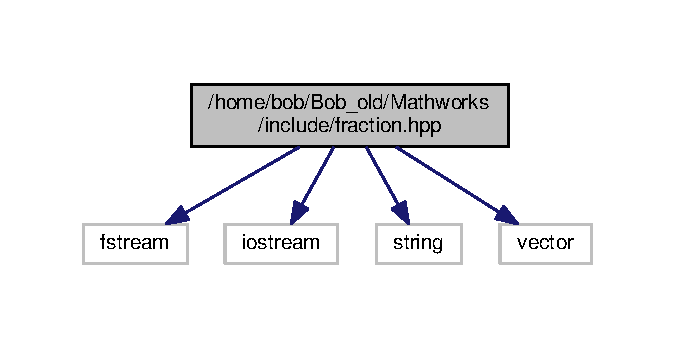
\includegraphics[width=324pt]{fraction_8hpp__incl}
\end{center}
\end{figure}
This graph shows which files directly or indirectly include this file\+:
\nopagebreak
\begin{figure}[H]
\begin{center}
\leavevmode
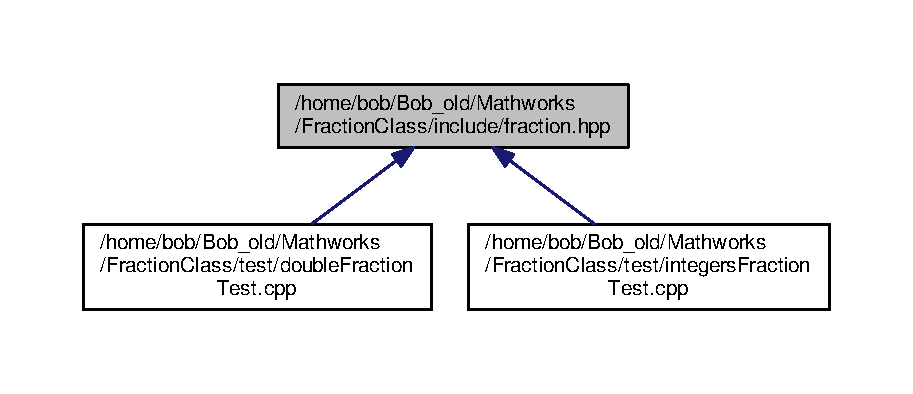
\includegraphics[width=350pt]{fraction_8hpp__dep__incl}
\end{center}
\end{figure}
\subsection*{Classes}
\begin{DoxyCompactItemize}
\item 
class \hyperlink{classfraction}{fraction$<$ T $>$}
\begin{DoxyCompactList}\small\item\em Fraction class declaration mentioning all members. \end{DoxyCompactList}\item 
class \hyperlink{classfraction}{fraction$<$ T $>$}
\begin{DoxyCompactList}\small\item\em Fraction class declaration mentioning all members. \end{DoxyCompactList}\end{DoxyCompactItemize}
\subsection*{Functions}
\begin{DoxyCompactItemize}
\item 
{\footnotesize template$<$typename T $>$ }\\T \hyperlink{fraction_8hpp_a843a3f34ca879eba5e52c3ec841d0597}{find\+Remainder} (T, T)
\begin{DoxyCompactList}\small\item\em To find the Remainder if first is divided by second, Used subtraction method to find remainder(mod). \end{DoxyCompactList}\item 
{\footnotesize template$<$typename T $>$ }\\T \hyperlink{fraction_8hpp_ad71ce5d79457e67a200307c8e7955c45}{greatest\+Common\+Divisor} (const T \&, const T \&)
\begin{DoxyCompactList}\small\item\em To find greatest common. \end{DoxyCompactList}\item 
{\footnotesize template$<$typename T $>$ }\\\hyperlink{classfraction}{fraction}$<$ T $>$ \hyperlink{fraction_8hpp_a63ec63f05cd3a1548da7d2ff00fd60a6}{operator+} (const \hyperlink{classfraction}{fraction}$<$ T $>$ \&first, const \hyperlink{classfraction}{fraction}$<$ T $>$ \&second)
\begin{DoxyCompactList}\small\item\em overloading operators + declaration \end{DoxyCompactList}\item 
{\footnotesize template$<$typename T $>$ }\\\hyperlink{classfraction}{fraction}$<$ T $>$ \hyperlink{fraction_8hpp_a6bdad9f1c32bf6e641b9fa5f70ee92fe}{operator-\/} (const \hyperlink{classfraction}{fraction}$<$ T $>$ \&first, const \hyperlink{classfraction}{fraction}$<$ T $>$ \&second)
\begin{DoxyCompactList}\small\item\em overloading operator -\/ declaration \end{DoxyCompactList}\item 
{\footnotesize template$<$typename T $>$ }\\\hyperlink{classfraction}{fraction}$<$ T $>$ \hyperlink{fraction_8hpp_aa44c78d4b034f5f70496ad76b71d15e6}{operator$\ast$} (const \hyperlink{classfraction}{fraction}$<$ T $>$ \&first, const \hyperlink{classfraction}{fraction}$<$ T $>$ \&second)
\begin{DoxyCompactList}\small\item\em overloading operator $\ast$ declaration \end{DoxyCompactList}\item 
{\footnotesize template$<$typename T $>$ }\\\hyperlink{classfraction}{fraction}$<$ T $>$ \hyperlink{fraction_8hpp_a4ad8f4a937536a26072298f08f2d29a3}{operator/} (const \hyperlink{classfraction}{fraction}$<$ T $>$ \&first, const \hyperlink{classfraction}{fraction}$<$ T $>$ \&second)
\begin{DoxyCompactList}\small\item\em overloading operator / declaration \end{DoxyCompactList}\item 
{\footnotesize template$<$typename T $>$ }\\\hyperlink{classfraction}{fraction}$<$ T $>$ \hyperlink{fraction_8hpp_ad50510e81993145c4a159dd0c0968b37}{operator+} (const T \&first, const \hyperlink{classfraction}{fraction}$<$ T $>$ \&second)
\begin{DoxyCompactList}\small\item\em overloading operator + for \{ T + fraction$<$\+T$>$ \} \end{DoxyCompactList}\item 
{\footnotesize template$<$typename T $>$ }\\\hyperlink{classfraction}{fraction}$<$ T $>$ \hyperlink{fraction_8hpp_a235606bd56c80c0e12e93a19b64179bd}{operator-\/} (const T \&first, const \hyperlink{classfraction}{fraction}$<$ T $>$ \&second)
\begin{DoxyCompactList}\small\item\em overloading operator -\/ for \{ T -\/ fraction$<$\+T$>$ \} \end{DoxyCompactList}\item 
{\footnotesize template$<$typename T $>$ }\\\hyperlink{classfraction}{fraction}$<$ T $>$ \hyperlink{fraction_8hpp_a3d501d68d95cb7008ad0b05406ff7368}{operator$\ast$} (const T \&first, const \hyperlink{classfraction}{fraction}$<$ T $>$ \&second)
\begin{DoxyCompactList}\small\item\em overloading operator $\ast$ for \{ T $\ast$ fraction$<$\+T$>$ \} \end{DoxyCompactList}\item 
{\footnotesize template$<$typename T $>$ }\\\hyperlink{classfraction}{fraction}$<$ T $>$ \hyperlink{fraction_8hpp_adf9dfd8d68f78355438c33529bbd1c88}{operator/} (const T \&first, const \hyperlink{classfraction}{fraction}$<$ T $>$ \&second)
\begin{DoxyCompactList}\small\item\em overloading operator / for \{ T / fraction$<$\+T$>$ \} \end{DoxyCompactList}\item 
{\footnotesize template$<$typename T $>$ }\\\hyperlink{classfraction}{fraction}$<$ T $>$ \hyperlink{fraction_8hpp_a2d31a24abb6f50cf03361e81c0cb6e97}{operator+} (const \hyperlink{classfraction}{fraction}$<$ T $>$ \&first, const T \&second)
\begin{DoxyCompactList}\small\item\em overloading operator + for \{ fraction$<$\+T$>$ + T\} \end{DoxyCompactList}\item 
{\footnotesize template$<$typename T $>$ }\\\hyperlink{classfraction}{fraction}$<$ T $>$ \hyperlink{fraction_8hpp_ae7405eff3703533e3e7158473b4d16ca}{operator-\/} (const \hyperlink{classfraction}{fraction}$<$ T $>$ \&first, const T \&second)
\begin{DoxyCompactList}\small\item\em overloading operator -\/ for \{ fraction$<$\+T$>$ -\/ T\} \end{DoxyCompactList}\item 
{\footnotesize template$<$typename T $>$ }\\\hyperlink{classfraction}{fraction}$<$ T $>$ \hyperlink{fraction_8hpp_a5344425f39764cd0008ef48e39d86466}{operator$\ast$} (const \hyperlink{classfraction}{fraction}$<$ T $>$ \&first, const T \&second)
\begin{DoxyCompactList}\small\item\em overloading operator $\ast$ for \{ fraction$<$\+T$>$ $\ast$ T\} \end{DoxyCompactList}\item 
{\footnotesize template$<$typename T $>$ }\\\hyperlink{classfraction}{fraction}$<$ T $>$ \hyperlink{fraction_8hpp_a78e3d561c8c49d0bb80b202afbd80a41}{operator/} (const \hyperlink{classfraction}{fraction}$<$ T $>$ \&first, const T \&second)
\begin{DoxyCompactList}\small\item\em overloading operator / for \{ fraction$<$\+T$>$ / T\} \end{DoxyCompactList}\item 
{\footnotesize template$<$typename T $>$ }\\\hyperlink{classfraction}{fraction}$<$ T $>$ \hyperlink{fraction_8hpp_a8763c0072913cd82ee9f8be262cf422b}{operator==} (const \hyperlink{classfraction}{fraction}$<$ T $>$ \&first, const \hyperlink{classfraction}{fraction}$<$ T $>$ \&second)
\begin{DoxyCompactList}\small\item\em overloading operator == to check equality of two fractions \end{DoxyCompactList}\item 
{\footnotesize template$<$typename T $>$ }\\\hyperlink{classfraction}{fraction}$<$ T $>$ \hyperlink{fraction_8hpp_a0449744962aa88a73382c2871c1a5b00}{operator!=} (const \hyperlink{classfraction}{fraction}$<$ T $>$ \&first, const \hyperlink{classfraction}{fraction}$<$ T $>$ \&second)
\begin{DoxyCompactList}\small\item\em overloading operator != to check non equality of two fractions \end{DoxyCompactList}\item 
{\footnotesize template$<$typename T $>$ }\\\hyperlink{classfraction}{fraction}$<$ T $>$ \hyperlink{fraction_8hpp_a6d2beade4eb826a0b3695c8c492dde8e}{operator$>$} (const \hyperlink{classfraction}{fraction}$<$ T $>$ \&first, const \hyperlink{classfraction}{fraction}$<$ T $>$ \&second)
\begin{DoxyCompactList}\small\item\em overloading operator $>$ to check which is greated between two fractions \end{DoxyCompactList}\item 
{\footnotesize template$<$typename T $>$ }\\\hyperlink{classfraction}{fraction}$<$ T $>$ \hyperlink{fraction_8hpp_a51e8d0e60240e3a41321965f3fb36e52}{operator$<$} (const \hyperlink{classfraction}{fraction}$<$ T $>$ \&first, const \hyperlink{classfraction}{fraction}$<$ T $>$ \&second)
\begin{DoxyCompactList}\small\item\em overloading operator $<$ to check which is lesser between two fractions \end{DoxyCompactList}\item 
{\footnotesize template$<$typename T $>$ }\\\hyperlink{classfraction}{fraction}$<$ T $>$ \hyperlink{fraction_8hpp_a257b033efb453e12d60e2a5a24c860b9}{operator==} (const \hyperlink{classfraction}{fraction}$<$ T $>$ \&first, const T \&second)
\begin{DoxyCompactList}\small\item\em overloading operator == to check equality of fraction$<$\+T$>$ and T \end{DoxyCompactList}\item 
{\footnotesize template$<$typename T $>$ }\\\hyperlink{classfraction}{fraction}$<$ T $>$ \hyperlink{fraction_8hpp_a34f1701d9564e522c0472fa798bb3d5d}{operator!=} (const \hyperlink{classfraction}{fraction}$<$ T $>$ \&first, const T \&second)
\begin{DoxyCompactList}\small\item\em overloading operator != to check equality of fraction$<$\+T$>$ and T \end{DoxyCompactList}\item 
{\footnotesize template$<$typename T $>$ }\\\hyperlink{classfraction}{fraction}$<$ T $>$ \hyperlink{fraction_8hpp_a7d7306b7591dd945b71db482a8c5799b}{operator$>$} (const \hyperlink{classfraction}{fraction}$<$ T $>$ \&first, const T \&second)
\begin{DoxyCompactList}\small\item\em overloading operator $>$ to check if fraction$<$\+T$>$ is greated than T \end{DoxyCompactList}\item 
{\footnotesize template$<$typename T $>$ }\\\hyperlink{classfraction}{fraction}$<$ T $>$ \hyperlink{fraction_8hpp_ac94fc22f63d770d0ab927b4cd194ee17}{operator$<$} (const \hyperlink{classfraction}{fraction}$<$ T $>$ \&first, const T \&second)
\begin{DoxyCompactList}\small\item\em overloading operator $<$ to check if fraction$<$\+T$>$ is lesser than T \end{DoxyCompactList}\item 
{\footnotesize template$<$typename T $>$ }\\\hyperlink{classfraction}{fraction}$<$ T $>$ \hyperlink{fraction_8hpp_a2e1cb02a82c29ba5c055e3f630894164}{operator==} (const T \&first, const \hyperlink{classfraction}{fraction}$<$ T $>$ \&second)
\begin{DoxyCompactList}\small\item\em overloading operator == to check equality of T and fraction$<$\+T$>$ \end{DoxyCompactList}\item 
{\footnotesize template$<$typename T $>$ }\\\hyperlink{classfraction}{fraction}$<$ T $>$ \hyperlink{fraction_8hpp_a7391546cf9ebc5565da0daed9780427f}{operator!=} (const T \&first, const \hyperlink{classfraction}{fraction}$<$ T $>$ \&second)
\begin{DoxyCompactList}\small\item\em overloading operator != to check equality of T and fraction$<$\+T$>$ \end{DoxyCompactList}\item 
{\footnotesize template$<$typename T $>$ }\\\hyperlink{classfraction}{fraction}$<$ T $>$ \hyperlink{fraction_8hpp_ab8efd15417e43c2c474be4e0b8e30db4}{operator$>$} (const T \&first, const \hyperlink{classfraction}{fraction}$<$ T $>$ \&second)
\begin{DoxyCompactList}\small\item\em overloading operator $>$ to check if T is greater than fraction$<$\+T$>$ \end{DoxyCompactList}\item 
{\footnotesize template$<$typename T $>$ }\\\hyperlink{classfraction}{fraction}$<$ T $>$ \hyperlink{fraction_8hpp_a6417ca69c17d57f1c27207292c1c1d6d}{operator$<$} (const T \&first, const \hyperlink{classfraction}{fraction}$<$ T $>$ \&second)
\begin{DoxyCompactList}\small\item\em overloading operator $<$ to check if T is less than fraction$<$\+T$>$ \end{DoxyCompactList}\item 
{\footnotesize template$<$typename T $>$ }\\std\+::ostream \& \hyperlink{fraction_8hpp_a8a44cb508a0d50b317a2c2cee120d96b}{operator$<$$<$} (std\+::ostream \&out, const \hyperlink{classfraction}{fraction}$<$ T $>$ \&a)
\begin{DoxyCompactList}\small\item\em overloading operator $>$$>$ to show output using ostream \end{DoxyCompactList}\item 
{\footnotesize template$<$typename T $>$ }\\std\+::istream \& \hyperlink{fraction_8hpp_a52ef4af97bcb6db6f6ec71c2781e3e69}{operator$>$$>$} (std\+::istream \&in, \hyperlink{classfraction}{fraction}$<$ T $>$ \&a)
\begin{DoxyCompactList}\small\item\em overloading $<$$<$ operator for input \end{DoxyCompactList}\item 
{\footnotesize template$<$typename T $>$ }\\bool \hyperlink{fraction_8hpp_ae258c0505616fd872a06cf5ff2255a20}{operator==} (\hyperlink{classfraction}{fraction}$<$ T $>$ \&first, \hyperlink{classfraction}{fraction}$<$ T $>$ \&second)
\begin{DoxyCompactList}\small\item\em equality comparision of a/b and c/d , they are equal when simplified versions have same numerator and denominator \end{DoxyCompactList}\item 
{\footnotesize template$<$typename T $>$ }\\bool \hyperlink{fraction_8hpp_a869713580aa3d3cb0576b1c291a33efa}{operator==} (\hyperlink{classfraction}{fraction}$<$ T $>$ \&first, const T \&second)
\begin{DoxyCompactList}\small\item\em a/b == c \end{DoxyCompactList}\item 
{\footnotesize template$<$typename T $>$ }\\bool \hyperlink{fraction_8hpp_ad36531e9a0a6ce02ca01db9d4b072e37}{operator==} (const T \&first, \hyperlink{classfraction}{fraction}$<$ T $>$ \&second)
\begin{DoxyCompactList}\small\item\em a == c/d \end{DoxyCompactList}\item 
{\footnotesize template$<$typename T $>$ }\\bool \hyperlink{fraction_8hpp_a93f8f1b9bfb0e92bda88f20d590b6d4b}{operator!=} (\hyperlink{classfraction}{fraction}$<$ T $>$ \&first, \hyperlink{classfraction}{fraction}$<$ T $>$ \&second)
\begin{DoxyCompactList}\small\item\em a/b != c/d equality check for two fractions \end{DoxyCompactList}\item 
{\footnotesize template$<$typename T $>$ }\\bool \hyperlink{fraction_8hpp_a93d4e34fcfb6818490f8a439d560c049}{operator!=} (\hyperlink{classfraction}{fraction}$<$ T $>$ \&first, const T \&second)
\begin{DoxyCompactList}\small\item\em a/b != c \end{DoxyCompactList}\item 
{\footnotesize template$<$typename T $>$ }\\bool \hyperlink{fraction_8hpp_a161bd870d7335786dea8358347be8803}{operator!=} (const T \&first, \hyperlink{classfraction}{fraction}$<$ T $>$ \&second)
\begin{DoxyCompactList}\small\item\em a != c/d \end{DoxyCompactList}\item 
{\footnotesize template$<$typename T $>$ }\\bool \hyperlink{fraction_8hpp_a1798ecef70ab99cd74218f29cdc90b68}{operator$>$} (\hyperlink{classfraction}{fraction}$<$ T $>$ \&first, \hyperlink{classfraction}{fraction}$<$ T $>$ \&second)
\begin{DoxyCompactList}\small\item\em check which one is bigger fraction a/b $>$ c/d a/b -\/ c/d $>$ 0 =$>$ ad -\/bc $>$ 0 =$>$ a/b is bigger than c/d \end{DoxyCompactList}\item 
{\footnotesize template$<$typename T $>$ }\\bool \hyperlink{fraction_8hpp_a2f7dbd3340051e09786eb7d183f215d2}{operator$>$} (\hyperlink{classfraction}{fraction}$<$ T $>$ \&first, const T \&second)
\begin{DoxyCompactList}\small\item\em check which one is bigger fraction a/b $>$ c a/b -\/ c $>$ 0 =$>$ a -\/bc $>$ 0 =$>$ a/b is bigger than c \end{DoxyCompactList}\item 
{\footnotesize template$<$typename T $>$ }\\bool \hyperlink{fraction_8hpp_ad09f2b840a04f5592734b2dc49a78a98}{operator$>$} (T \&first, \hyperlink{classfraction}{fraction}$<$ T $>$ \&second)
\begin{DoxyCompactList}\small\item\em check which one is bigger fraction a/b $>$ c/d a -\/ c/d $>$ 0 =$>$ ad -\/c $>$ 0 =$>$ a is bigger than c/d \end{DoxyCompactList}\item 
{\footnotesize template$<$typename T $>$ }\\bool \hyperlink{fraction_8hpp_ad0ace2e2114c6b41de426a4f4505eca3}{operator$<$} (\hyperlink{classfraction}{fraction}$<$ T $>$ \&first, \hyperlink{classfraction}{fraction}$<$ T $>$ \&second)
\begin{DoxyCompactList}\small\item\em check which one is smaller fraction a/b $<$ c/d a/b -\/ c/d $>$ 0 =$>$ ad -\/bc $>$ 0 =$>$ c/d is lesser than a/b \end{DoxyCompactList}\item 
{\footnotesize template$<$typename T $>$ }\\bool \hyperlink{fraction_8hpp_a53c6efebd40ef67d99ef9dc2b3bd940a}{operator$<$} (\hyperlink{classfraction}{fraction}$<$ T $>$ \&first, const T \&second)
\begin{DoxyCompactList}\small\item\em check which one is smaller fraction a/b $<$ c a/b -\/ c $>$ 0 =$>$ a -\/bc $>$ 0 =$>$ c is lesser than a/b \end{DoxyCompactList}\item 
{\footnotesize template$<$typename T $>$ }\\bool \hyperlink{fraction_8hpp_afab3e36727df8b80931454c2b8f123c3}{operator$<$} (const T \&first, \hyperlink{classfraction}{fraction}$<$ T $>$ \&second)
\begin{DoxyCompactList}\small\item\em check which one is smaller fraction a$<$ c/d a -\/ c/d $>$ 0 =$>$ ad -\/c $>$ 0 =$>$ c/d is lesser than a \end{DoxyCompactList}\end{DoxyCompactItemize}


\subsection{Detailed Description}
Fraction Class file with definitions and declarations, (generally definitions and declarations should be separated in different files, here using templates to define/declare functions) Overloaded addition, subtraction,multiply,division,greater/lesser than,equality/non equality operators to perform appropriate actions with fractions.\+Also has display function and overloaded $>$$>$ and $<$$<$ functions to show output and get input respectively. Also includes find\+Remainder and greatest Common divisor function. 

\begin{DoxyAuthor}{Author}
Bhargav Dandamudi 
\end{DoxyAuthor}
\begin{DoxyVersion}{Version}
1 
\end{DoxyVersion}
\begin{DoxyDate}{Date}
2019-\/04-\/18 
\end{DoxyDate}


\subsection{Function Documentation}
\index{fraction.\+hpp@{fraction.\+hpp}!find\+Remainder@{find\+Remainder}}
\index{find\+Remainder@{find\+Remainder}!fraction.\+hpp@{fraction.\+hpp}}
\subsubsection[{\texorpdfstring{find\+Remainder(\+T, T)}{findRemainder(T, T)}}]{\setlength{\rightskip}{0pt plus 5cm}template$<$typename T $>$ T find\+Remainder (
\begin{DoxyParamCaption}
\item[{T}]{first, }
\item[{T}]{second}
\end{DoxyParamCaption}
)}\hypertarget{fraction_8hpp_a843a3f34ca879eba5e52c3ec841d0597}{}\label{fraction_8hpp_a843a3f34ca879eba5e52c3ec841d0597}


To find the Remainder if first is divided by second, Used subtraction method to find remainder(mod). 

Finding remainder using subtraction method, subract until we get negative value, not using const and \& , as we are changing values.


\begin{DoxyParams}{Parameters}
{\em T} & first number (dividend) \\
\hline
{\em T} & second number (divisor)\\
\hline
\end{DoxyParams}
\begin{DoxyReturn}{Returns}
remainder
\end{DoxyReturn}

\begin{DoxyTemplParams}{Template Parameters}
{\em T} & \\
\hline
\end{DoxyTemplParams}

\begin{DoxyParams}{Parameters}
{\em first} & \\
\hline
{\em second} & \\
\hline
\end{DoxyParams}
\begin{DoxyReturn}{Returns}
remainder if first is divided by second 
\end{DoxyReturn}
\index{fraction.\+hpp@{fraction.\+hpp}!greatest\+Common\+Divisor@{greatest\+Common\+Divisor}}
\index{greatest\+Common\+Divisor@{greatest\+Common\+Divisor}!fraction.\+hpp@{fraction.\+hpp}}
\subsubsection[{\texorpdfstring{greatest\+Common\+Divisor(const T \&, const T \&)}{greatestCommonDivisor(const T &, const T &)}}]{\setlength{\rightskip}{0pt plus 5cm}template$<$typename T $>$ T greatest\+Common\+Divisor (
\begin{DoxyParamCaption}
\item[{const T \&}]{numerator, }
\item[{const T \&}]{denominator}
\end{DoxyParamCaption}
)}\hypertarget{fraction_8hpp_ad71ce5d79457e67a200307c8e7955c45}{}\label{fraction_8hpp_ad71ce5d79457e67a200307c8e7955c45}


To find greatest common. 

To G\+CD of two numbers using euclids algorithm, recursive method.


\begin{DoxyParams}{Parameters}
{\em input} & number one \\
\hline
{\em input} & number two\\
\hline
\end{DoxyParams}
\begin{DoxyReturn}{Returns}
greatest common divisor for number one and two
\end{DoxyReturn}

\begin{DoxyTemplParams}{Template Parameters}
{\em T} & \\
\hline
\end{DoxyTemplParams}

\begin{DoxyParams}{Parameters}
{\em numerator} & \\
\hline
{\em denominator} & \\
\hline
\end{DoxyParams}
\begin{DoxyReturn}{Returns}
number of type T with G\+CD value 
\end{DoxyReturn}
\index{fraction.\+hpp@{fraction.\+hpp}!operator"!=@{operator"!=}}
\index{operator"!=@{operator"!=}!fraction.\+hpp@{fraction.\+hpp}}
\subsubsection[{\texorpdfstring{operator"!=(const fraction$<$ T $>$ \&first, const fraction$<$ T $>$ \&second)}{operator!=(const fraction< T > &first, const fraction< T > &second)}}]{\setlength{\rightskip}{0pt plus 5cm}template$<$typename T $>$ {\bf fraction}$<$T$>$ operator!= (
\begin{DoxyParamCaption}
\item[{const {\bf fraction}$<$ T $>$ \&}]{first, }
\item[{const {\bf fraction}$<$ T $>$ \&}]{second}
\end{DoxyParamCaption}
)}\hypertarget{fraction_8hpp_a0449744962aa88a73382c2871c1a5b00}{}\label{fraction_8hpp_a0449744962aa88a73382c2871c1a5b00}


overloading operator != to check non equality of two fractions 


\begin{DoxyTemplParams}{Template Parameters}
{\em T} & \\
\hline
\end{DoxyTemplParams}

\begin{DoxyParams}{Parameters}
{\em first} & \\
\hline
{\em second} & \\
\hline
\end{DoxyParams}
\begin{DoxyReturn}{Returns}
bool true if not equal else false 
\end{DoxyReturn}
\index{fraction.\+hpp@{fraction.\+hpp}!operator"!=@{operator"!=}}
\index{operator"!=@{operator"!=}!fraction.\+hpp@{fraction.\+hpp}}
\subsubsection[{\texorpdfstring{operator"!=(const fraction$<$ T $>$ \&first, const T \&second)}{operator!=(const fraction< T > &first, const T &second)}}]{\setlength{\rightskip}{0pt plus 5cm}template$<$typename T $>$ {\bf fraction}$<$T$>$ operator!= (
\begin{DoxyParamCaption}
\item[{const {\bf fraction}$<$ T $>$ \&}]{first, }
\item[{const T \&}]{second}
\end{DoxyParamCaption}
)}\hypertarget{fraction_8hpp_a34f1701d9564e522c0472fa798bb3d5d}{}\label{fraction_8hpp_a34f1701d9564e522c0472fa798bb3d5d}


overloading operator != to check equality of fraction$<$\+T$>$ and T 


\begin{DoxyTemplParams}{Template Parameters}
{\em T} & template parameter \\
\hline
\end{DoxyTemplParams}

\begin{DoxyParams}{Parameters}
{\em first} & \\
\hline
{\em second} & \\
\hline
\end{DoxyParams}
\begin{DoxyReturn}{Returns}
false of fraction$<$\+T$>$ and T are equal else true 
\end{DoxyReturn}
\index{fraction.\+hpp@{fraction.\+hpp}!operator"!=@{operator"!=}}
\index{operator"!=@{operator"!=}!fraction.\+hpp@{fraction.\+hpp}}
\subsubsection[{\texorpdfstring{operator"!=(const T \&first, const fraction$<$ T $>$ \&second)}{operator!=(const T &first, const fraction< T > &second)}}]{\setlength{\rightskip}{0pt plus 5cm}template$<$typename T $>$ {\bf fraction}$<$T$>$ operator!= (
\begin{DoxyParamCaption}
\item[{const T \&}]{first, }
\item[{const {\bf fraction}$<$ T $>$ \&}]{second}
\end{DoxyParamCaption}
)}\hypertarget{fraction_8hpp_a7391546cf9ebc5565da0daed9780427f}{}\label{fraction_8hpp_a7391546cf9ebc5565da0daed9780427f}


overloading operator != to check equality of T and fraction$<$\+T$>$ 


\begin{DoxyTemplParams}{Template Parameters}
{\em T} & template parameter \\
\hline
\end{DoxyTemplParams}

\begin{DoxyParams}{Parameters}
{\em first} & \\
\hline
{\em second} & \\
\hline
\end{DoxyParams}
\begin{DoxyReturn}{Returns}
false if fraction$<$\+T$>$ and T are equal else true 
\end{DoxyReturn}
\index{fraction.\+hpp@{fraction.\+hpp}!operator"!=@{operator"!=}}
\index{operator"!=@{operator"!=}!fraction.\+hpp@{fraction.\+hpp}}
\subsubsection[{\texorpdfstring{operator"!=(fraction$<$ T $>$ \&first, fraction$<$ T $>$ \&second)}{operator!=(fraction< T > &first, fraction< T > &second)}}]{\setlength{\rightskip}{0pt plus 5cm}template$<$typename T $>$ bool operator!= (
\begin{DoxyParamCaption}
\item[{{\bf fraction}$<$ T $>$ \&}]{first, }
\item[{{\bf fraction}$<$ T $>$ \&}]{second}
\end{DoxyParamCaption}
)}\hypertarget{fraction_8hpp_a93f8f1b9bfb0e92bda88f20d590b6d4b}{}\label{fraction_8hpp_a93f8f1b9bfb0e92bda88f20d590b6d4b}


a/b != c/d equality check for two fractions 


\begin{DoxyTemplParams}{Template Parameters}
{\em T} & \\
\hline
\end{DoxyTemplParams}

\begin{DoxyParams}{Parameters}
{\em first} & a/b \\
\hline
{\em second} & c/d\\
\hline
\end{DoxyParams}
\begin{DoxyReturn}{Returns}
false if equal else true 
\end{DoxyReturn}
\index{fraction.\+hpp@{fraction.\+hpp}!operator"!=@{operator"!=}}
\index{operator"!=@{operator"!=}!fraction.\+hpp@{fraction.\+hpp}}
\subsubsection[{\texorpdfstring{operator"!=(fraction$<$ T $>$ \&first, const T \&second)}{operator!=(fraction< T > &first, const T &second)}}]{\setlength{\rightskip}{0pt plus 5cm}template$<$typename T $>$ bool operator!= (
\begin{DoxyParamCaption}
\item[{{\bf fraction}$<$ T $>$ \&}]{first, }
\item[{const T \&}]{second}
\end{DoxyParamCaption}
)}\hypertarget{fraction_8hpp_a93d4e34fcfb6818490f8a439d560c049}{}\label{fraction_8hpp_a93d4e34fcfb6818490f8a439d560c049}


a/b != c 


\begin{DoxyTemplParams}{Template Parameters}
{\em T} & \\
\hline
\end{DoxyTemplParams}

\begin{DoxyParams}{Parameters}
{\em first} & a/b \\
\hline
{\em second} & c\\
\hline
\end{DoxyParams}
\begin{DoxyReturn}{Returns}
false if equal else true 
\end{DoxyReturn}
\index{fraction.\+hpp@{fraction.\+hpp}!operator"!=@{operator"!=}}
\index{operator"!=@{operator"!=}!fraction.\+hpp@{fraction.\+hpp}}
\subsubsection[{\texorpdfstring{operator"!=(const T \&first, fraction$<$ T $>$ \&second)}{operator!=(const T &first, fraction< T > &second)}}]{\setlength{\rightskip}{0pt plus 5cm}template$<$typename T $>$ bool operator!= (
\begin{DoxyParamCaption}
\item[{const T \&}]{first, }
\item[{{\bf fraction}$<$ T $>$ \&}]{second}
\end{DoxyParamCaption}
)}\hypertarget{fraction_8hpp_a161bd870d7335786dea8358347be8803}{}\label{fraction_8hpp_a161bd870d7335786dea8358347be8803}


a != c/d 


\begin{DoxyTemplParams}{Template Parameters}
{\em T} & \\
\hline
\end{DoxyTemplParams}

\begin{DoxyParams}{Parameters}
{\em first} & a \\
\hline
{\em second} & c/d\\
\hline
\end{DoxyParams}
\begin{DoxyReturn}{Returns}
true if not equal else false 
\end{DoxyReturn}
\index{fraction.\+hpp@{fraction.\+hpp}!operator$\ast$@{operator$\ast$}}
\index{operator$\ast$@{operator$\ast$}!fraction.\+hpp@{fraction.\+hpp}}
\subsubsection[{\texorpdfstring{operator$\ast$(const fraction$<$ T $>$ \&first, const fraction$<$ T $>$ \&second)}{operator*(const fraction< T > &first, const fraction< T > &second)}}]{\setlength{\rightskip}{0pt plus 5cm}template$<$typename T $>$ {\bf fraction}$<$ T $>$ operator$\ast$ (
\begin{DoxyParamCaption}
\item[{const {\bf fraction}$<$ T $>$ \&}]{first, }
\item[{const {\bf fraction}$<$ T $>$ \&}]{second}
\end{DoxyParamCaption}
)}\hypertarget{fraction_8hpp_aa44c78d4b034f5f70496ad76b71d15e6}{}\label{fraction_8hpp_aa44c78d4b034f5f70496ad76b71d15e6}


overloading operator $\ast$ declaration 

product of two fractions a/b $\ast$ c/d = ac/bd


\begin{DoxyTemplParams}{Template Parameters}
{\em T} & template parameter \\
\hline
\end{DoxyTemplParams}

\begin{DoxyParams}{Parameters}
{\em first} & \\
\hline
{\em second} & \\
\hline
\end{DoxyParams}
\begin{DoxyReturn}{Returns}
product of two input fractions
\end{DoxyReturn}

\begin{DoxyTemplParams}{Template Parameters}
{\em T} & \\
\hline
\end{DoxyTemplParams}

\begin{DoxyParams}{Parameters}
{\em first} & a/b \\
\hline
{\em second} & c/d\\
\hline
\end{DoxyParams}
\begin{DoxyReturn}{Returns}
product 
\end{DoxyReturn}
\index{fraction.\+hpp@{fraction.\+hpp}!operator$\ast$@{operator$\ast$}}
\index{operator$\ast$@{operator$\ast$}!fraction.\+hpp@{fraction.\+hpp}}
\subsubsection[{\texorpdfstring{operator$\ast$(const T \&first, const fraction$<$ T $>$ \&second)}{operator*(const T &first, const fraction< T > &second)}}]{\setlength{\rightskip}{0pt plus 5cm}template$<$typename T $>$ {\bf fraction}$<$ T $>$ operator$\ast$ (
\begin{DoxyParamCaption}
\item[{const T \&}]{first, }
\item[{const {\bf fraction}$<$ T $>$ \&}]{second}
\end{DoxyParamCaption}
)}\hypertarget{fraction_8hpp_a3d501d68d95cb7008ad0b05406ff7368}{}\label{fraction_8hpp_a3d501d68d95cb7008ad0b05406ff7368}


overloading operator $\ast$ for \{ T $\ast$ fraction$<$\+T$>$ \} 

a $\ast$ c/d = ac/d


\begin{DoxyParams}{Parameters}
{\em first} & \\
\hline
{\em second} & \\
\hline
\end{DoxyParams}
\begin{DoxyReturn}{Returns}
product of T and fraction$<$\+T$>$
\end{DoxyReturn}

\begin{DoxyTemplParams}{Template Parameters}
{\em T} & \\
\hline
\end{DoxyTemplParams}

\begin{DoxyParams}{Parameters}
{\em first} & a \\
\hline
{\em second} & c/d\\
\hline
\end{DoxyParams}
\begin{DoxyReturn}{Returns}
product 
\end{DoxyReturn}
\index{fraction.\+hpp@{fraction.\+hpp}!operator$\ast$@{operator$\ast$}}
\index{operator$\ast$@{operator$\ast$}!fraction.\+hpp@{fraction.\+hpp}}
\subsubsection[{\texorpdfstring{operator$\ast$(const fraction$<$ T $>$ \&first, const T \&second)}{operator*(const fraction< T > &first, const T &second)}}]{\setlength{\rightskip}{0pt plus 5cm}template$<$typename T $>$ {\bf fraction}$<$ T $>$ operator$\ast$ (
\begin{DoxyParamCaption}
\item[{const {\bf fraction}$<$ T $>$ \&}]{first, }
\item[{const T \&}]{second}
\end{DoxyParamCaption}
)}\hypertarget{fraction_8hpp_a5344425f39764cd0008ef48e39d86466}{}\label{fraction_8hpp_a5344425f39764cd0008ef48e39d86466}


overloading operator $\ast$ for \{ fraction$<$\+T$>$ $\ast$ T\} 

a/b $\ast$ c


\begin{DoxyTemplParams}{Template Parameters}
{\em T} & \\
\hline
\end{DoxyTemplParams}

\begin{DoxyParams}{Parameters}
{\em first} & \\
\hline
{\em second} & \\
\hline
\end{DoxyParams}
\begin{DoxyReturn}{Returns}
product of fraction$<$\+T$>$ and T
\end{DoxyReturn}

\begin{DoxyTemplParams}{Template Parameters}
{\em T} & \\
\hline
\end{DoxyTemplParams}

\begin{DoxyParams}{Parameters}
{\em first} & a/b \\
\hline
{\em second} & c\\
\hline
\end{DoxyParams}
\begin{DoxyReturn}{Returns}
product 
\end{DoxyReturn}
\index{fraction.\+hpp@{fraction.\+hpp}!operator+@{operator+}}
\index{operator+@{operator+}!fraction.\+hpp@{fraction.\+hpp}}
\subsubsection[{\texorpdfstring{operator+(const fraction$<$ T $>$ \&first, const fraction$<$ T $>$ \&second)}{operator+(const fraction< T > &first, const fraction< T > &second)}}]{\setlength{\rightskip}{0pt plus 5cm}template$<$typename T $>$ {\bf fraction}$<$ T $>$ operator+ (
\begin{DoxyParamCaption}
\item[{const {\bf fraction}$<$ T $>$ \&}]{first, }
\item[{const {\bf fraction}$<$ T $>$ \&}]{second}
\end{DoxyParamCaption}
)}\hypertarget{fraction_8hpp_a63ec63f05cd3a1548da7d2ff00fd60a6}{}\label{fraction_8hpp_a63ec63f05cd3a1548da7d2ff00fd60a6}


overloading operators + declaration 

addition of fractions a/b + c/d = (a$\ast$d +b$\ast$c)/ (bd)


\begin{DoxyTemplParams}{Template Parameters}
{\em T} & template parameter \\
\hline
\end{DoxyTemplParams}

\begin{DoxyParams}{Parameters}
{\em first} & \\
\hline
{\em second} & \\
\hline
\end{DoxyParams}
\begin{DoxyReturn}{Returns}
sum of two fractions
\end{DoxyReturn}

\begin{DoxyParams}{Parameters}
{\em first} & \\
\hline
{\em second} & \\
\hline
\end{DoxyParams}
\begin{DoxyReturn}{Returns}
sum 
\end{DoxyReturn}
\index{fraction.\+hpp@{fraction.\+hpp}!operator+@{operator+}}
\index{operator+@{operator+}!fraction.\+hpp@{fraction.\+hpp}}
\subsubsection[{\texorpdfstring{operator+(const T \&first, const fraction$<$ T $>$ \&second)}{operator+(const T &first, const fraction< T > &second)}}]{\setlength{\rightskip}{0pt plus 5cm}template$<$typename T $>$ {\bf fraction}$<$ T $>$ operator+ (
\begin{DoxyParamCaption}
\item[{const T \&}]{first, }
\item[{const {\bf fraction}$<$ T $>$ \&}]{second}
\end{DoxyParamCaption}
)}\hypertarget{fraction_8hpp_ad50510e81993145c4a159dd0c0968b37}{}\label{fraction_8hpp_ad50510e81993145c4a159dd0c0968b37}


overloading operator + for \{ T + fraction$<$\+T$>$ \} 

a + c/d


\begin{DoxyParams}{Parameters}
{\em first} & \\
\hline
{\em second} & \\
\hline
\end{DoxyParams}
\begin{DoxyReturn}{Returns}
sum of T and fraction$<$\+T$>$
\end{DoxyReturn}

\begin{DoxyTemplParams}{Template Parameters}
{\em T} & \\
\hline
\end{DoxyTemplParams}

\begin{DoxyParams}{Parameters}
{\em first} & a \\
\hline
{\em second} & c/d\\
\hline
\end{DoxyParams}
\begin{DoxyReturn}{Returns}
sum 
\end{DoxyReturn}
\index{fraction.\+hpp@{fraction.\+hpp}!operator+@{operator+}}
\index{operator+@{operator+}!fraction.\+hpp@{fraction.\+hpp}}
\subsubsection[{\texorpdfstring{operator+(const fraction$<$ T $>$ \&first, const T \&second)}{operator+(const fraction< T > &first, const T &second)}}]{\setlength{\rightskip}{0pt plus 5cm}template$<$typename T $>$ {\bf fraction}$<$ T $>$ operator+ (
\begin{DoxyParamCaption}
\item[{const {\bf fraction}$<$ T $>$ \&}]{first, }
\item[{const T \&}]{second}
\end{DoxyParamCaption}
)}\hypertarget{fraction_8hpp_a2d31a24abb6f50cf03361e81c0cb6e97}{}\label{fraction_8hpp_a2d31a24abb6f50cf03361e81c0cb6e97}


overloading operator + for \{ fraction$<$\+T$>$ + T\} 

a/b + c


\begin{DoxyTemplParams}{Template Parameters}
{\em T} & \\
\hline
\end{DoxyTemplParams}

\begin{DoxyParams}{Parameters}
{\em first} & \\
\hline
{\em second} & \\
\hline
\end{DoxyParams}
\begin{DoxyReturn}{Returns}
sum of fraction$<$\+T$>$ and T
\end{DoxyReturn}

\begin{DoxyTemplParams}{Template Parameters}
{\em T} & \\
\hline
\end{DoxyTemplParams}

\begin{DoxyParams}{Parameters}
{\em first} & \\
\hline
{\em second} & \\
\hline
\end{DoxyParams}
\begin{DoxyReturn}{Returns}
sum 
\end{DoxyReturn}
\index{fraction.\+hpp@{fraction.\+hpp}!operator-\/@{operator-\/}}
\index{operator-\/@{operator-\/}!fraction.\+hpp@{fraction.\+hpp}}
\subsubsection[{\texorpdfstring{operator-\/(const fraction$<$ T $>$ \&first, const fraction$<$ T $>$ \&second)}{operator-(const fraction< T > &first, const fraction< T > &second)}}]{\setlength{\rightskip}{0pt plus 5cm}template$<$typename T $>$ {\bf fraction}$<$ T $>$ operator-\/ (
\begin{DoxyParamCaption}
\item[{const {\bf fraction}$<$ T $>$ \&}]{first, }
\item[{const {\bf fraction}$<$ T $>$ \&}]{second}
\end{DoxyParamCaption}
)}\hypertarget{fraction_8hpp_a6bdad9f1c32bf6e641b9fa5f70ee92fe}{}\label{fraction_8hpp_a6bdad9f1c32bf6e641b9fa5f70ee92fe}


overloading operator -\/ declaration 

a/b -\/ c/d = (ad -\/ bc) /bd ;difference


\begin{DoxyTemplParams}{Template Parameters}
{\em T} & template parameter \\
\hline
\end{DoxyTemplParams}

\begin{DoxyParams}{Parameters}
{\em first} & \\
\hline
{\em second} & \\
\hline
\end{DoxyParams}
\begin{DoxyReturn}{Returns}
difference of two input fractions
\end{DoxyReturn}

\begin{DoxyTemplParams}{Template Parameters}
{\em T} & \\
\hline
\end{DoxyTemplParams}

\begin{DoxyParams}{Parameters}
{\em first} & a/b \\
\hline
{\em second} & c/d\\
\hline
\end{DoxyParams}
\begin{DoxyReturn}{Returns}
difference 
\end{DoxyReturn}
\index{fraction.\+hpp@{fraction.\+hpp}!operator-\/@{operator-\/}}
\index{operator-\/@{operator-\/}!fraction.\+hpp@{fraction.\+hpp}}
\subsubsection[{\texorpdfstring{operator-\/(const T \&first, const fraction$<$ T $>$ \&second)}{operator-(const T &first, const fraction< T > &second)}}]{\setlength{\rightskip}{0pt plus 5cm}template$<$typename T $>$ {\bf fraction}$<$ T $>$ operator-\/ (
\begin{DoxyParamCaption}
\item[{const T \&}]{first, }
\item[{const {\bf fraction}$<$ T $>$ \&}]{second}
\end{DoxyParamCaption}
)}\hypertarget{fraction_8hpp_a235606bd56c80c0e12e93a19b64179bd}{}\label{fraction_8hpp_a235606bd56c80c0e12e93a19b64179bd}


overloading operator -\/ for \{ T -\/ fraction$<$\+T$>$ \} 

a -\/c/d


\begin{DoxyParams}{Parameters}
{\em first} & \\
\hline
{\em second} & \\
\hline
\end{DoxyParams}
\begin{DoxyReturn}{Returns}
difference of T and fraction$<$\+T$>$
\end{DoxyReturn}

\begin{DoxyTemplParams}{Template Parameters}
{\em T} & \\
\hline
\end{DoxyTemplParams}

\begin{DoxyParams}{Parameters}
{\em first} & \\
\hline
{\em second} & \\
\hline
\end{DoxyParams}
\begin{DoxyReturn}{Returns}
difference 
\end{DoxyReturn}
\index{fraction.\+hpp@{fraction.\+hpp}!operator-\/@{operator-\/}}
\index{operator-\/@{operator-\/}!fraction.\+hpp@{fraction.\+hpp}}
\subsubsection[{\texorpdfstring{operator-\/(const fraction$<$ T $>$ \&first, const T \&second)}{operator-(const fraction< T > &first, const T &second)}}]{\setlength{\rightskip}{0pt plus 5cm}template$<$typename T $>$ {\bf fraction}$<$ T $>$ operator-\/ (
\begin{DoxyParamCaption}
\item[{const {\bf fraction}$<$ T $>$ \&}]{first, }
\item[{const T \&}]{second}
\end{DoxyParamCaption}
)}\hypertarget{fraction_8hpp_ae7405eff3703533e3e7158473b4d16ca}{}\label{fraction_8hpp_ae7405eff3703533e3e7158473b4d16ca}


overloading operator -\/ for \{ fraction$<$\+T$>$ -\/ T\} 

a/b -\/c


\begin{DoxyTemplParams}{Template Parameters}
{\em T} & \\
\hline
\end{DoxyTemplParams}

\begin{DoxyParams}{Parameters}
{\em first} & \\
\hline
{\em second} & \\
\hline
\end{DoxyParams}
\begin{DoxyReturn}{Returns}
difference of fraction$<$\+T$>$ and T
\end{DoxyReturn}

\begin{DoxyTemplParams}{Template Parameters}
{\em T} & \\
\hline
\end{DoxyTemplParams}

\begin{DoxyParams}{Parameters}
{\em first} & \\
\hline
{\em second} & \\
\hline
\end{DoxyParams}
\begin{DoxyReturn}{Returns}
difference 
\end{DoxyReturn}
\index{fraction.\+hpp@{fraction.\+hpp}!operator/@{operator/}}
\index{operator/@{operator/}!fraction.\+hpp@{fraction.\+hpp}}
\subsubsection[{\texorpdfstring{operator/(const fraction$<$ T $>$ \&first, const fraction$<$ T $>$ \&second)}{operator/(const fraction< T > &first, const fraction< T > &second)}}]{\setlength{\rightskip}{0pt plus 5cm}template$<$typename T $>$ {\bf fraction}$<$ T $>$ operator/ (
\begin{DoxyParamCaption}
\item[{const {\bf fraction}$<$ T $>$ \&}]{first, }
\item[{const {\bf fraction}$<$ T $>$ \&}]{second}
\end{DoxyParamCaption}
)}\hypertarget{fraction_8hpp_a4ad8f4a937536a26072298f08f2d29a3}{}\label{fraction_8hpp_a4ad8f4a937536a26072298f08f2d29a3}


overloading operator / declaration 

division of two fraction (a/b) / (c/d) = a$\ast$d / b$\ast$c


\begin{DoxyTemplParams}{Template Parameters}
{\em T} & template parameter \\
\hline
\end{DoxyTemplParams}

\begin{DoxyParams}{Parameters}
{\em first} & \\
\hline
{\em second} & \\
\hline
\end{DoxyParams}
\begin{DoxyReturn}{Returns}
division of two input fractions
\end{DoxyReturn}

\begin{DoxyTemplParams}{Template Parameters}
{\em T} & \\
\hline
\end{DoxyTemplParams}

\begin{DoxyParams}{Parameters}
{\em first} & a/b \\
\hline
{\em second} & c/d\\
\hline
\end{DoxyParams}
\begin{DoxyReturn}{Returns}
ad/bc division 
\end{DoxyReturn}
\index{fraction.\+hpp@{fraction.\+hpp}!operator/@{operator/}}
\index{operator/@{operator/}!fraction.\+hpp@{fraction.\+hpp}}
\subsubsection[{\texorpdfstring{operator/(const T \&first, const fraction$<$ T $>$ \&second)}{operator/(const T &first, const fraction< T > &second)}}]{\setlength{\rightskip}{0pt plus 5cm}template$<$typename T $>$ {\bf fraction}$<$ T $>$ operator/ (
\begin{DoxyParamCaption}
\item[{const T \&}]{first, }
\item[{const {\bf fraction}$<$ T $>$ \&}]{second}
\end{DoxyParamCaption}
)}\hypertarget{fraction_8hpp_adf9dfd8d68f78355438c33529bbd1c88}{}\label{fraction_8hpp_adf9dfd8d68f78355438c33529bbd1c88}


overloading operator / for \{ T / fraction$<$\+T$>$ \} 

a / (c/d) = ad/c


\begin{DoxyParams}{Parameters}
{\em first} & \\
\hline
{\em second} & \\
\hline
\end{DoxyParams}
\begin{DoxyReturn}{Returns}
division of T and fraction$<$\+T$>$
\end{DoxyReturn}

\begin{DoxyTemplParams}{Template Parameters}
{\em T} & \\
\hline
\end{DoxyTemplParams}

\begin{DoxyParams}{Parameters}
{\em first} & a \\
\hline
{\em second} & c/d\\
\hline
\end{DoxyParams}
\begin{DoxyReturn}{Returns}
ad/c division 
\end{DoxyReturn}
\index{fraction.\+hpp@{fraction.\+hpp}!operator/@{operator/}}
\index{operator/@{operator/}!fraction.\+hpp@{fraction.\+hpp}}
\subsubsection[{\texorpdfstring{operator/(const fraction$<$ T $>$ \&first, const T \&second)}{operator/(const fraction< T > &first, const T &second)}}]{\setlength{\rightskip}{0pt plus 5cm}template$<$typename T $>$ {\bf fraction}$<$ T $>$ operator/ (
\begin{DoxyParamCaption}
\item[{const {\bf fraction}$<$ T $>$ \&}]{first, }
\item[{const T \&}]{second}
\end{DoxyParamCaption}
)}\hypertarget{fraction_8hpp_a78e3d561c8c49d0bb80b202afbd80a41}{}\label{fraction_8hpp_a78e3d561c8c49d0bb80b202afbd80a41}


overloading operator / for \{ fraction$<$\+T$>$ / T\} 

a/b / c = a/bc


\begin{DoxyTemplParams}{Template Parameters}
{\em T} & \\
\hline
\end{DoxyTemplParams}

\begin{DoxyParams}{Parameters}
{\em first} & \\
\hline
{\em second} & \\
\hline
\end{DoxyParams}
\begin{DoxyReturn}{Returns}
division of fraction$<$\+T$>$ and T
\end{DoxyReturn}

\begin{DoxyTemplParams}{Template Parameters}
{\em T} & \\
\hline
\end{DoxyTemplParams}

\begin{DoxyParams}{Parameters}
{\em first} & a/b \\
\hline
{\em second} & c/1\\
\hline
\end{DoxyParams}
\begin{DoxyReturn}{Returns}
a/bc division 
\end{DoxyReturn}
\index{fraction.\+hpp@{fraction.\+hpp}!operator$<$@{operator$<$}}
\index{operator$<$@{operator$<$}!fraction.\+hpp@{fraction.\+hpp}}
\subsubsection[{\texorpdfstring{operator$<$(const fraction$<$ T $>$ \&first, const fraction$<$ T $>$ \&second)}{operator<(const fraction< T > &first, const fraction< T > &second)}}]{\setlength{\rightskip}{0pt plus 5cm}template$<$typename T $>$ {\bf fraction}$<$T$>$ operator$<$ (
\begin{DoxyParamCaption}
\item[{const {\bf fraction}$<$ T $>$ \&}]{first, }
\item[{const {\bf fraction}$<$ T $>$ \&}]{second}
\end{DoxyParamCaption}
)}\hypertarget{fraction_8hpp_a51e8d0e60240e3a41321965f3fb36e52}{}\label{fraction_8hpp_a51e8d0e60240e3a41321965f3fb36e52}


overloading operator $<$ to check which is lesser between two fractions 


\begin{DoxyTemplParams}{Template Parameters}
{\em T} & \\
\hline
\end{DoxyTemplParams}

\begin{DoxyParams}{Parameters}
{\em first} & \\
\hline
{\em second} & \\
\hline
\end{DoxyParams}
\begin{DoxyReturn}{Returns}
bool true if first is less than second else false 
\end{DoxyReturn}
\index{fraction.\+hpp@{fraction.\+hpp}!operator$<$@{operator$<$}}
\index{operator$<$@{operator$<$}!fraction.\+hpp@{fraction.\+hpp}}
\subsubsection[{\texorpdfstring{operator$<$(const fraction$<$ T $>$ \&first, const T \&second)}{operator<(const fraction< T > &first, const T &second)}}]{\setlength{\rightskip}{0pt plus 5cm}template$<$typename T $>$ {\bf fraction}$<$T$>$ operator$<$ (
\begin{DoxyParamCaption}
\item[{const {\bf fraction}$<$ T $>$ \&}]{first, }
\item[{const T \&}]{second}
\end{DoxyParamCaption}
)}\hypertarget{fraction_8hpp_ac94fc22f63d770d0ab927b4cd194ee17}{}\label{fraction_8hpp_ac94fc22f63d770d0ab927b4cd194ee17}


overloading operator $<$ to check if fraction$<$\+T$>$ is lesser than T 


\begin{DoxyTemplParams}{Template Parameters}
{\em T} & template parameter \\
\hline
\end{DoxyTemplParams}

\begin{DoxyParams}{Parameters}
{\em first} & \\
\hline
{\em second} & \\
\hline
\end{DoxyParams}
\begin{DoxyReturn}{Returns}
true if fraction$<$\+T$>$ is less than T else false 
\end{DoxyReturn}
\index{fraction.\+hpp@{fraction.\+hpp}!operator$<$@{operator$<$}}
\index{operator$<$@{operator$<$}!fraction.\+hpp@{fraction.\+hpp}}
\subsubsection[{\texorpdfstring{operator$<$(const T \&first, const fraction$<$ T $>$ \&second)}{operator<(const T &first, const fraction< T > &second)}}]{\setlength{\rightskip}{0pt plus 5cm}template$<$typename T $>$ {\bf fraction}$<$T$>$ operator$<$ (
\begin{DoxyParamCaption}
\item[{const T \&}]{first, }
\item[{const {\bf fraction}$<$ T $>$ \&}]{second}
\end{DoxyParamCaption}
)}\hypertarget{fraction_8hpp_a6417ca69c17d57f1c27207292c1c1d6d}{}\label{fraction_8hpp_a6417ca69c17d57f1c27207292c1c1d6d}


overloading operator $<$ to check if T is less than fraction$<$\+T$>$ 


\begin{DoxyTemplParams}{Template Parameters}
{\em T} & template parameter \\
\hline
\end{DoxyTemplParams}

\begin{DoxyParams}{Parameters}
{\em first} & \\
\hline
{\em second} & \\
\hline
\end{DoxyParams}
\begin{DoxyReturn}{Returns}
true if T is less than fraction$<$\+T$>$ else false 
\end{DoxyReturn}
\index{fraction.\+hpp@{fraction.\+hpp}!operator$<$@{operator$<$}}
\index{operator$<$@{operator$<$}!fraction.\+hpp@{fraction.\+hpp}}
\subsubsection[{\texorpdfstring{operator$<$(fraction$<$ T $>$ \&first, fraction$<$ T $>$ \&second)}{operator<(fraction< T > &first, fraction< T > &second)}}]{\setlength{\rightskip}{0pt plus 5cm}template$<$typename T $>$ bool operator$<$ (
\begin{DoxyParamCaption}
\item[{{\bf fraction}$<$ T $>$ \&}]{first, }
\item[{{\bf fraction}$<$ T $>$ \&}]{second}
\end{DoxyParamCaption}
)}\hypertarget{fraction_8hpp_ad0ace2e2114c6b41de426a4f4505eca3}{}\label{fraction_8hpp_ad0ace2e2114c6b41de426a4f4505eca3}


check which one is smaller fraction a/b $<$ c/d a/b -\/ c/d $>$ 0 =$>$ ad -\/bc $>$ 0 =$>$ c/d is lesser than a/b 


\begin{DoxyTemplParams}{Template Parameters}
{\em T} & \\
\hline
\end{DoxyTemplParams}

\begin{DoxyParams}{Parameters}
{\em first} & a/b \\
\hline
{\em second} & c/d\\
\hline
\end{DoxyParams}
\begin{DoxyReturn}{Returns}
true if first is smaller else false 
\end{DoxyReturn}
\index{fraction.\+hpp@{fraction.\+hpp}!operator$<$@{operator$<$}}
\index{operator$<$@{operator$<$}!fraction.\+hpp@{fraction.\+hpp}}
\subsubsection[{\texorpdfstring{operator$<$(fraction$<$ T $>$ \&first, const T \&second)}{operator<(fraction< T > &first, const T &second)}}]{\setlength{\rightskip}{0pt plus 5cm}template$<$typename T $>$ bool operator$<$ (
\begin{DoxyParamCaption}
\item[{{\bf fraction}$<$ T $>$ \&}]{first, }
\item[{const T \&}]{second}
\end{DoxyParamCaption}
)}\hypertarget{fraction_8hpp_a53c6efebd40ef67d99ef9dc2b3bd940a}{}\label{fraction_8hpp_a53c6efebd40ef67d99ef9dc2b3bd940a}


check which one is smaller fraction a/b $<$ c a/b -\/ c $>$ 0 =$>$ a -\/bc $>$ 0 =$>$ c is lesser than a/b 


\begin{DoxyTemplParams}{Template Parameters}
{\em T} & \\
\hline
\end{DoxyTemplParams}

\begin{DoxyParams}{Parameters}
{\em first} & a/b \\
\hline
{\em second} & c/d\\
\hline
\end{DoxyParams}
\begin{DoxyReturn}{Returns}
true if first is smaller else false 
\end{DoxyReturn}
\index{fraction.\+hpp@{fraction.\+hpp}!operator$<$@{operator$<$}}
\index{operator$<$@{operator$<$}!fraction.\+hpp@{fraction.\+hpp}}
\subsubsection[{\texorpdfstring{operator$<$(const T \&first, fraction$<$ T $>$ \&second)}{operator<(const T &first, fraction< T > &second)}}]{\setlength{\rightskip}{0pt plus 5cm}template$<$typename T $>$ bool operator$<$ (
\begin{DoxyParamCaption}
\item[{const T \&}]{first, }
\item[{{\bf fraction}$<$ T $>$ \&}]{second}
\end{DoxyParamCaption}
)}\hypertarget{fraction_8hpp_afab3e36727df8b80931454c2b8f123c3}{}\label{fraction_8hpp_afab3e36727df8b80931454c2b8f123c3}


check which one is smaller fraction a$<$ c/d a -\/ c/d $>$ 0 =$>$ ad -\/c $>$ 0 =$>$ c/d is lesser than a 


\begin{DoxyTemplParams}{Template Parameters}
{\em T} & \\
\hline
\end{DoxyTemplParams}

\begin{DoxyParams}{Parameters}
{\em first} & a/b \\
\hline
{\em second} & c/d\\
\hline
\end{DoxyParams}
\begin{DoxyReturn}{Returns}
true if first is smaller else false 
\end{DoxyReturn}
\index{fraction.\+hpp@{fraction.\+hpp}!operator$<$$<$@{operator$<$$<$}}
\index{operator$<$$<$@{operator$<$$<$}!fraction.\+hpp@{fraction.\+hpp}}
\subsubsection[{\texorpdfstring{operator$<$$<$(std\+::ostream \&out, const fraction$<$ T $>$ \&a)}{operator<<(std::ostream &out, const fraction< T > &a)}}]{\setlength{\rightskip}{0pt plus 5cm}template$<$typename T $>$ std\+::ostream \& operator$<$$<$ (
\begin{DoxyParamCaption}
\item[{std\+::ostream \&}]{out, }
\item[{const {\bf fraction}$<$ T $>$ \&}]{fraction}
\end{DoxyParamCaption}
)}\hypertarget{fraction_8hpp_a8a44cb508a0d50b317a2c2cee120d96b}{}\label{fraction_8hpp_a8a44cb508a0d50b317a2c2cee120d96b}


overloading operator $>$$>$ to show output using ostream 

TO show output in ostream.


\begin{DoxyTemplParams}{Template Parameters}
{\em T} & \\
\hline
\end{DoxyTemplParams}

\begin{DoxyParams}{Parameters}
{\em out} & \\
\hline
{\em a} & \\
\hline
\end{DoxyParams}
\begin{DoxyReturn}{Returns}
ostream if we have any output fraction to be shown
\end{DoxyReturn}

\begin{DoxyTemplParams}{Template Parameters}
{\em T} & \\
\hline
\end{DoxyTemplParams}

\begin{DoxyParams}{Parameters}
{\em out} & \\
\hline
{\em fraction} & \\
\hline
\end{DoxyParams}
\begin{DoxyReturn}{Returns}
ostream 
\end{DoxyReturn}
\index{fraction.\+hpp@{fraction.\+hpp}!operator==@{operator==}}
\index{operator==@{operator==}!fraction.\+hpp@{fraction.\+hpp}}
\subsubsection[{\texorpdfstring{operator==(const fraction$<$ T $>$ \&first, const fraction$<$ T $>$ \&second)}{operator==(const fraction< T > &first, const fraction< T > &second)}}]{\setlength{\rightskip}{0pt plus 5cm}template$<$typename T $>$ {\bf fraction}$<$T$>$ operator== (
\begin{DoxyParamCaption}
\item[{const {\bf fraction}$<$ T $>$ \&}]{first, }
\item[{const {\bf fraction}$<$ T $>$ \&}]{second}
\end{DoxyParamCaption}
)}\hypertarget{fraction_8hpp_a8763c0072913cd82ee9f8be262cf422b}{}\label{fraction_8hpp_a8763c0072913cd82ee9f8be262cf422b}


overloading operator == to check equality of two fractions 


\begin{DoxyTemplParams}{Template Parameters}
{\em T} & \\
\hline
\end{DoxyTemplParams}

\begin{DoxyParams}{Parameters}
{\em first} & \\
\hline
{\em second} & \\
\hline
\end{DoxyParams}
\begin{DoxyReturn}{Returns}
bool true if equal else false 
\end{DoxyReturn}
\index{fraction.\+hpp@{fraction.\+hpp}!operator==@{operator==}}
\index{operator==@{operator==}!fraction.\+hpp@{fraction.\+hpp}}
\subsubsection[{\texorpdfstring{operator==(const fraction$<$ T $>$ \&first, const T \&second)}{operator==(const fraction< T > &first, const T &second)}}]{\setlength{\rightskip}{0pt plus 5cm}template$<$typename T $>$ {\bf fraction}$<$T$>$ operator== (
\begin{DoxyParamCaption}
\item[{const {\bf fraction}$<$ T $>$ \&}]{first, }
\item[{const T \&}]{second}
\end{DoxyParamCaption}
)}\hypertarget{fraction_8hpp_a257b033efb453e12d60e2a5a24c860b9}{}\label{fraction_8hpp_a257b033efb453e12d60e2a5a24c860b9}


overloading operator == to check equality of fraction$<$\+T$>$ and T 


\begin{DoxyTemplParams}{Template Parameters}
{\em T} & template parameter \\
\hline
\end{DoxyTemplParams}

\begin{DoxyParams}{Parameters}
{\em first} & \\
\hline
{\em second} & \\
\hline
\end{DoxyParams}
\begin{DoxyReturn}{Returns}
true of fraction$<$\+T$>$ and T are equal 
\end{DoxyReturn}
\index{fraction.\+hpp@{fraction.\+hpp}!operator==@{operator==}}
\index{operator==@{operator==}!fraction.\+hpp@{fraction.\+hpp}}
\subsubsection[{\texorpdfstring{operator==(const T \&first, const fraction$<$ T $>$ \&second)}{operator==(const T &first, const fraction< T > &second)}}]{\setlength{\rightskip}{0pt plus 5cm}template$<$typename T $>$ {\bf fraction}$<$T$>$ operator== (
\begin{DoxyParamCaption}
\item[{const T \&}]{first, }
\item[{const {\bf fraction}$<$ T $>$ \&}]{second}
\end{DoxyParamCaption}
)}\hypertarget{fraction_8hpp_a2e1cb02a82c29ba5c055e3f630894164}{}\label{fraction_8hpp_a2e1cb02a82c29ba5c055e3f630894164}


overloading operator == to check equality of T and fraction$<$\+T$>$ 


\begin{DoxyTemplParams}{Template Parameters}
{\em T} & template parameter \\
\hline
\end{DoxyTemplParams}

\begin{DoxyParams}{Parameters}
{\em first} & \\
\hline
{\em second} & \\
\hline
\end{DoxyParams}
\begin{DoxyReturn}{Returns}
true if fraction$<$\+T$>$ and T are equal 
\end{DoxyReturn}
\index{fraction.\+hpp@{fraction.\+hpp}!operator==@{operator==}}
\index{operator==@{operator==}!fraction.\+hpp@{fraction.\+hpp}}
\subsubsection[{\texorpdfstring{operator==(fraction$<$ T $>$ \&first, fraction$<$ T $>$ \&second)}{operator==(fraction< T > &first, fraction< T > &second)}}]{\setlength{\rightskip}{0pt plus 5cm}template$<$typename T $>$ bool operator== (
\begin{DoxyParamCaption}
\item[{{\bf fraction}$<$ T $>$ \&}]{first, }
\item[{{\bf fraction}$<$ T $>$ \&}]{second}
\end{DoxyParamCaption}
)}\hypertarget{fraction_8hpp_ae258c0505616fd872a06cf5ff2255a20}{}\label{fraction_8hpp_ae258c0505616fd872a06cf5ff2255a20}


equality comparision of a/b and c/d , they are equal when simplified versions have same numerator and denominator 


\begin{DoxyTemplParams}{Template Parameters}
{\em T} & \\
\hline
\end{DoxyTemplParams}

\begin{DoxyParams}{Parameters}
{\em first} & a/b \\
\hline
{\em second} & c/d\\
\hline
\end{DoxyParams}
\begin{DoxyReturn}{Returns}
true if equal else false 
\end{DoxyReturn}
\index{fraction.\+hpp@{fraction.\+hpp}!operator==@{operator==}}
\index{operator==@{operator==}!fraction.\+hpp@{fraction.\+hpp}}
\subsubsection[{\texorpdfstring{operator==(fraction$<$ T $>$ \&first, const T \&second)}{operator==(fraction< T > &first, const T &second)}}]{\setlength{\rightskip}{0pt plus 5cm}template$<$typename T $>$ bool operator== (
\begin{DoxyParamCaption}
\item[{{\bf fraction}$<$ T $>$ \&}]{first, }
\item[{const T \&}]{second}
\end{DoxyParamCaption}
)}\hypertarget{fraction_8hpp_a869713580aa3d3cb0576b1c291a33efa}{}\label{fraction_8hpp_a869713580aa3d3cb0576b1c291a33efa}


a/b == c 


\begin{DoxyTemplParams}{Template Parameters}
{\em T} & \\
\hline
\end{DoxyTemplParams}

\begin{DoxyParams}{Parameters}
{\em first} & a/b \\
\hline
{\em second} & c\\
\hline
\end{DoxyParams}
\begin{DoxyReturn}{Returns}
true if equal else false 
\end{DoxyReturn}
\index{fraction.\+hpp@{fraction.\+hpp}!operator==@{operator==}}
\index{operator==@{operator==}!fraction.\+hpp@{fraction.\+hpp}}
\subsubsection[{\texorpdfstring{operator==(const T \&first, fraction$<$ T $>$ \&second)}{operator==(const T &first, fraction< T > &second)}}]{\setlength{\rightskip}{0pt plus 5cm}template$<$typename T $>$ bool operator== (
\begin{DoxyParamCaption}
\item[{const T \&}]{first, }
\item[{{\bf fraction}$<$ T $>$ \&}]{second}
\end{DoxyParamCaption}
)}\hypertarget{fraction_8hpp_ad36531e9a0a6ce02ca01db9d4b072e37}{}\label{fraction_8hpp_ad36531e9a0a6ce02ca01db9d4b072e37}


a == c/d 


\begin{DoxyTemplParams}{Template Parameters}
{\em T} & \\
\hline
\end{DoxyTemplParams}

\begin{DoxyParams}{Parameters}
{\em first} & a \\
\hline
{\em second} & c/d\\
\hline
\end{DoxyParams}
\begin{DoxyReturn}{Returns}
true if equal else false 
\end{DoxyReturn}
\index{fraction.\+hpp@{fraction.\+hpp}!operator$>$@{operator$>$}}
\index{operator$>$@{operator$>$}!fraction.\+hpp@{fraction.\+hpp}}
\subsubsection[{\texorpdfstring{operator$>$(const fraction$<$ T $>$ \&first, const fraction$<$ T $>$ \&second)}{operator>(const fraction< T > &first, const fraction< T > &second)}}]{\setlength{\rightskip}{0pt plus 5cm}template$<$typename T $>$ {\bf fraction}$<$T$>$ operator$>$ (
\begin{DoxyParamCaption}
\item[{const {\bf fraction}$<$ T $>$ \&}]{first, }
\item[{const {\bf fraction}$<$ T $>$ \&}]{second}
\end{DoxyParamCaption}
)}\hypertarget{fraction_8hpp_a6d2beade4eb826a0b3695c8c492dde8e}{}\label{fraction_8hpp_a6d2beade4eb826a0b3695c8c492dde8e}


overloading operator $>$ to check which is greated between two fractions 


\begin{DoxyTemplParams}{Template Parameters}
{\em T} & \\
\hline
\end{DoxyTemplParams}

\begin{DoxyParams}{Parameters}
{\em first} & \\
\hline
{\em second} & \\
\hline
\end{DoxyParams}
\begin{DoxyReturn}{Returns}
bool true if first is greater than second else false 
\end{DoxyReturn}
\index{fraction.\+hpp@{fraction.\+hpp}!operator$>$@{operator$>$}}
\index{operator$>$@{operator$>$}!fraction.\+hpp@{fraction.\+hpp}}
\subsubsection[{\texorpdfstring{operator$>$(const fraction$<$ T $>$ \&first, const T \&second)}{operator>(const fraction< T > &first, const T &second)}}]{\setlength{\rightskip}{0pt plus 5cm}template$<$typename T $>$ {\bf fraction}$<$T$>$ operator$>$ (
\begin{DoxyParamCaption}
\item[{const {\bf fraction}$<$ T $>$ \&}]{first, }
\item[{const T \&}]{second}
\end{DoxyParamCaption}
)}\hypertarget{fraction_8hpp_a7d7306b7591dd945b71db482a8c5799b}{}\label{fraction_8hpp_a7d7306b7591dd945b71db482a8c5799b}


overloading operator $>$ to check if fraction$<$\+T$>$ is greated than T 


\begin{DoxyTemplParams}{Template Parameters}
{\em T} & template parameter \\
\hline
\end{DoxyTemplParams}

\begin{DoxyParams}{Parameters}
{\em first} & \\
\hline
{\em second} & \\
\hline
\end{DoxyParams}
\begin{DoxyReturn}{Returns}
true of fraction$<$\+T$>$ is greater than T else false 
\end{DoxyReturn}
\index{fraction.\+hpp@{fraction.\+hpp}!operator$>$@{operator$>$}}
\index{operator$>$@{operator$>$}!fraction.\+hpp@{fraction.\+hpp}}
\subsubsection[{\texorpdfstring{operator$>$(const T \&first, const fraction$<$ T $>$ \&second)}{operator>(const T &first, const fraction< T > &second)}}]{\setlength{\rightskip}{0pt plus 5cm}template$<$typename T $>$ {\bf fraction}$<$T$>$ operator$>$ (
\begin{DoxyParamCaption}
\item[{const T \&}]{first, }
\item[{const {\bf fraction}$<$ T $>$ \&}]{second}
\end{DoxyParamCaption}
)}\hypertarget{fraction_8hpp_ab8efd15417e43c2c474be4e0b8e30db4}{}\label{fraction_8hpp_ab8efd15417e43c2c474be4e0b8e30db4}


overloading operator $>$ to check if T is greater than fraction$<$\+T$>$ 


\begin{DoxyTemplParams}{Template Parameters}
{\em T} & template parameter \\
\hline
\end{DoxyTemplParams}

\begin{DoxyParams}{Parameters}
{\em first} & \\
\hline
{\em second} & \\
\hline
\end{DoxyParams}
\begin{DoxyReturn}{Returns}
true if T is greater than fraction$<$\+T$>$ else false 
\end{DoxyReturn}
\index{fraction.\+hpp@{fraction.\+hpp}!operator$>$@{operator$>$}}
\index{operator$>$@{operator$>$}!fraction.\+hpp@{fraction.\+hpp}}
\subsubsection[{\texorpdfstring{operator$>$(fraction$<$ T $>$ \&first, fraction$<$ T $>$ \&second)}{operator>(fraction< T > &first, fraction< T > &second)}}]{\setlength{\rightskip}{0pt plus 5cm}template$<$typename T $>$ bool operator$>$ (
\begin{DoxyParamCaption}
\item[{{\bf fraction}$<$ T $>$ \&}]{first, }
\item[{{\bf fraction}$<$ T $>$ \&}]{second}
\end{DoxyParamCaption}
)}\hypertarget{fraction_8hpp_a1798ecef70ab99cd74218f29cdc90b68}{}\label{fraction_8hpp_a1798ecef70ab99cd74218f29cdc90b68}


check which one is bigger fraction a/b $>$ c/d a/b -\/ c/d $>$ 0 =$>$ ad -\/bc $>$ 0 =$>$ a/b is bigger than c/d 


\begin{DoxyTemplParams}{Template Parameters}
{\em T} & \\
\hline
\end{DoxyTemplParams}

\begin{DoxyParams}{Parameters}
{\em first} & a/b \\
\hline
{\em second} & c/d\\
\hline
\end{DoxyParams}
\begin{DoxyReturn}{Returns}
true if first is bigger else false 
\end{DoxyReturn}
\index{fraction.\+hpp@{fraction.\+hpp}!operator$>$@{operator$>$}}
\index{operator$>$@{operator$>$}!fraction.\+hpp@{fraction.\+hpp}}
\subsubsection[{\texorpdfstring{operator$>$(fraction$<$ T $>$ \&first, const T \&second)}{operator>(fraction< T > &first, const T &second)}}]{\setlength{\rightskip}{0pt plus 5cm}template$<$typename T $>$ bool operator$>$ (
\begin{DoxyParamCaption}
\item[{{\bf fraction}$<$ T $>$ \&}]{first, }
\item[{const T \&}]{second}
\end{DoxyParamCaption}
)}\hypertarget{fraction_8hpp_a2f7dbd3340051e09786eb7d183f215d2}{}\label{fraction_8hpp_a2f7dbd3340051e09786eb7d183f215d2}


check which one is bigger fraction a/b $>$ c a/b -\/ c $>$ 0 =$>$ a -\/bc $>$ 0 =$>$ a/b is bigger than c 


\begin{DoxyTemplParams}{Template Parameters}
{\em T} & \\
\hline
\end{DoxyTemplParams}

\begin{DoxyParams}{Parameters}
{\em first} & a/b \\
\hline
{\em second} & c\\
\hline
\end{DoxyParams}
\begin{DoxyReturn}{Returns}
true if first is bigger else false 
\end{DoxyReturn}
\index{fraction.\+hpp@{fraction.\+hpp}!operator$>$@{operator$>$}}
\index{operator$>$@{operator$>$}!fraction.\+hpp@{fraction.\+hpp}}
\subsubsection[{\texorpdfstring{operator$>$(\+T \&first, fraction$<$ T $>$ \&second)}{operator>(T &first, fraction< T > &second)}}]{\setlength{\rightskip}{0pt plus 5cm}template$<$typename T $>$ bool operator$>$ (
\begin{DoxyParamCaption}
\item[{T \&}]{first, }
\item[{{\bf fraction}$<$ T $>$ \&}]{second}
\end{DoxyParamCaption}
)}\hypertarget{fraction_8hpp_ad09f2b840a04f5592734b2dc49a78a98}{}\label{fraction_8hpp_ad09f2b840a04f5592734b2dc49a78a98}


check which one is bigger fraction a/b $>$ c/d a -\/ c/d $>$ 0 =$>$ ad -\/c $>$ 0 =$>$ a is bigger than c/d 


\begin{DoxyTemplParams}{Template Parameters}
{\em T} & \\
\hline
\end{DoxyTemplParams}

\begin{DoxyParams}{Parameters}
{\em first} & a \\
\hline
{\em second} & c/d\\
\hline
\end{DoxyParams}
\begin{DoxyReturn}{Returns}
true if first is bigger else false 
\end{DoxyReturn}
\index{fraction.\+hpp@{fraction.\+hpp}!operator$>$$>$@{operator$>$$>$}}
\index{operator$>$$>$@{operator$>$$>$}!fraction.\+hpp@{fraction.\+hpp}}
\subsubsection[{\texorpdfstring{operator$>$$>$(std\+::istream \&in, fraction$<$ T $>$ \&a)}{operator>>(std::istream &in, fraction< T > &a)}}]{\setlength{\rightskip}{0pt plus 5cm}template$<$typename T $>$ std\+::istream \& operator$>$$>$ (
\begin{DoxyParamCaption}
\item[{std\+::istream \&}]{in, }
\item[{{\bf fraction}$<$ T $>$ \&}]{fraction}
\end{DoxyParamCaption}
)}\hypertarget{fraction_8hpp_a52ef4af97bcb6db6f6ec71c2781e3e69}{}\label{fraction_8hpp_a52ef4af97bcb6db6f6ec71c2781e3e69}


overloading $<$$<$ operator for input 

To get input as fraction.


\begin{DoxyTemplParams}{Template Parameters}
{\em T} & \\
\hline
\end{DoxyTemplParams}

\begin{DoxyParams}{Parameters}
{\em in} & \\
\hline
{\em a} & \\
\hline
\end{DoxyParams}
\begin{DoxyReturn}{Returns}
istream if we need to input any fraction
\end{DoxyReturn}

\begin{DoxyTemplParams}{Template Parameters}
{\em T} & \\
\hline
\end{DoxyTemplParams}

\begin{DoxyParams}{Parameters}
{\em in} & \\
\hline
{\em fraction} & \\
\hline
\end{DoxyParams}
\begin{DoxyReturn}{Returns}
istream 
\end{DoxyReturn}

\hypertarget{doubleFractionTest_8cpp}{}\section{/home/bob/\+Bob\+\_\+old/\+Mathworks/test/double\+Fraction\+Test.cpp File Reference}
\label{doubleFractionTest_8cpp}\index{/home/bob/\+Bob\+\_\+old/\+Mathworks/test/double\+Fraction\+Test.\+cpp@{/home/bob/\+Bob\+\_\+old/\+Mathworks/test/double\+Fraction\+Test.\+cpp}}


Testing fraction class functions with double data type.  


{\ttfamily \#include \char`\"{}../include/fraction.\+hpp\char`\"{}}\\*
{\ttfamily \#include $<$gtest/gtest.\+h$>$}\\*
Include dependency graph for double\+Fraction\+Test.\+cpp\+:
\nopagebreak
\begin{figure}[H]
\begin{center}
\leavevmode
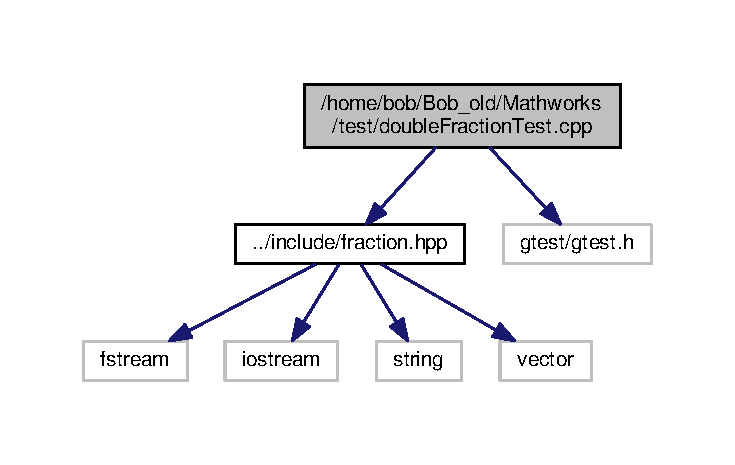
\includegraphics[width=350pt]{doubleFractionTest_8cpp__incl}
\end{center}
\end{figure}
\subsection*{Functions}
\begin{DoxyCompactItemize}
\item 
\hyperlink{doubleFractionTest_8cpp_a6cd3203f5fe8a50afd6aa99b70621d79}{T\+E\+ST} (Double\+Test, addition\+\_\+numerator)
\begin{DoxyCompactList}\small\item\em a/b +c/d \end{DoxyCompactList}\item 
{\bfseries T\+E\+ST} (Double\+Test, addition\+\_\+denominator)\hypertarget{doubleFractionTest_8cpp_ab1fdd318814056e7cdaf23aefe6f3a54}{}\label{doubleFractionTest_8cpp_ab1fdd318814056e7cdaf23aefe6f3a54}

\item 
\hyperlink{doubleFractionTest_8cpp_ab5d7fd0f213d9e57e851b7c19e3edc18}{T\+E\+ST} (Double\+Test, mixed\+\_\+addition\+\_\+nume)
\begin{DoxyCompactList}\small\item\em a/b +c ; c+a/b \end{DoxyCompactList}\item 
{\bfseries T\+E\+ST} (Double\+Test, mixed\+\_\+addition\+\_\+deno)\hypertarget{doubleFractionTest_8cpp_ac6ca627fa3bf94536bcd44c65947fd66}{}\label{doubleFractionTest_8cpp_ac6ca627fa3bf94536bcd44c65947fd66}

\item 
\hyperlink{doubleFractionTest_8cpp_a40e6086e840021d87e70d0f9015e4a94}{T\+E\+ST} (Double\+Test, subtraction\+\_\+numerator)
\begin{DoxyCompactList}\small\item\em a/b -\/c/d \end{DoxyCompactList}\item 
{\bfseries T\+E\+ST} (Double\+Test, subtraction\+\_\+deno)\hypertarget{doubleFractionTest_8cpp_abcfd44d3a0ddfa6813199983912f0b52}{}\label{doubleFractionTest_8cpp_abcfd44d3a0ddfa6813199983912f0b52}

\item 
\hyperlink{doubleFractionTest_8cpp_aa30d95b5c1c122c898df8e4f5ae4815a}{T\+E\+ST} (Double\+Test, mixed\+\_\+sub\+\_\+nume)
\begin{DoxyCompactList}\small\item\em a/b-\/c;c-\/a/b \end{DoxyCompactList}\item 
{\bfseries T\+E\+ST} (Double\+Test, mixed\+\_\+sub\+\_\+deno)\hypertarget{doubleFractionTest_8cpp_aa8ef35a515db45c05d54374164fedc4c}{}\label{doubleFractionTest_8cpp_aa8ef35a515db45c05d54374164fedc4c}

\item 
\hyperlink{doubleFractionTest_8cpp_aca2f2b36ee899e67d757aa30de745092}{T\+E\+ST} (Double\+Test, multiply\+\_\+test)
\begin{DoxyCompactList}\small\item\em a/b $\ast$ c/d \end{DoxyCompactList}\item 
{\bfseries T\+E\+ST} (Double\+Test, multiply\+\_\+mix\+\_\+test)\hypertarget{doubleFractionTest_8cpp_ac330beedc5afa652de1c68591154b69f}{}\label{doubleFractionTest_8cpp_ac330beedc5afa652de1c68591154b69f}

\item 
\hyperlink{doubleFractionTest_8cpp_a1207693372a307be789ef04fd30a7569}{T\+E\+ST} (Double\+Test, divide\+\_\+test)
\begin{DoxyCompactList}\small\item\em (a/b) / (c/d) \end{DoxyCompactList}\item 
\hyperlink{doubleFractionTest_8cpp_a0aec85683df9311179607a0b7218074b}{T\+E\+ST} (Double\+Test, divide\+\_\+mix\+\_\+test)
\begin{DoxyCompactList}\small\item\em a/b / (c) ; (c) / (a/b) \end{DoxyCompactList}\item 
\hyperlink{doubleFractionTest_8cpp_afacfb978b44caacb1020b259be446c71}{T\+E\+ST} (Double\+Test, greater\+\_\+test)
\begin{DoxyCompactList}\small\item\em a/b $>$ c/d \end{DoxyCompactList}\item 
\hyperlink{doubleFractionTest_8cpp_a116e264a741b048447630f4b51988f7b}{T\+E\+ST} (Double\+Test, greater\+\_\+mix\+\_\+test)
\begin{DoxyCompactList}\small\item\em a/b $>$ c; c $>$ a/b \end{DoxyCompactList}\item 
\hyperlink{doubleFractionTest_8cpp_a8fe1ed892babcd5e1c3d84abf94deee9}{T\+E\+ST} (Double\+Test, lesser\+\_\+test)
\begin{DoxyCompactList}\small\item\em a/b $<$ c/d \end{DoxyCompactList}\item 
\hyperlink{doubleFractionTest_8cpp_a08c830960b29879d34f2c38b0fece4f0}{T\+E\+ST} (Double\+Test, lesser\+\_\+mix\+\_\+test)
\begin{DoxyCompactList}\small\item\em a/b $<$ c; c$<$a/b \end{DoxyCompactList}\item 
\hyperlink{doubleFractionTest_8cpp_ac7ed905c83972991261afa8fcf9e528c}{T\+E\+ST} (Double\+Test, equality\+\_\+test)
\begin{DoxyCompactList}\small\item\em a/b == c/d \end{DoxyCompactList}\item 
\hyperlink{doubleFractionTest_8cpp_ac6eabc7bfe67f349fcd24a3b22fce247}{T\+E\+ST} (Double\+Test, equality\+Mix\+Test)
\begin{DoxyCompactList}\small\item\em a/b ==c;c==a/b \end{DoxyCompactList}\item 
\hyperlink{doubleFractionTest_8cpp_a14001a1f3eaf15d09a46893f61381dd6}{T\+E\+ST} (Double\+Test, not\+Equal\+Test)
\begin{DoxyCompactList}\small\item\em a/b !=c/d \end{DoxyCompactList}\item 
\hyperlink{doubleFractionTest_8cpp_a49ca28f6bb36127e6efeefabddb4cd3e}{T\+E\+ST} (Double\+Test, not\+Equal\+Mix\+Test)
\begin{DoxyCompactList}\small\item\em a/b !=c ;c!=a/b \end{DoxyCompactList}\end{DoxyCompactItemize}
\subsection*{Variables}
\begin{DoxyCompactItemize}
\item 
\hyperlink{classfraction}{fraction}$<$ double $>$ {\bfseries aa} (2, 4)\hypertarget{doubleFractionTest_8cpp_aba6b5fd30070c3b60c3211de5e367c8e}{}\label{doubleFractionTest_8cpp_aba6b5fd30070c3b60c3211de5e367c8e}

\item 
\hyperlink{classfraction}{fraction}$<$ double $>$ {\bfseries bb} (6, 8)\hypertarget{doubleFractionTest_8cpp_a69f641eff6d4d4988ad3cda5d5ef641d}{}\label{doubleFractionTest_8cpp_a69f641eff6d4d4988ad3cda5d5ef641d}

\end{DoxyCompactItemize}


\subsection{Detailed Description}
Testing fraction class functions with double data type. 

\begin{DoxyAuthor}{Author}
Bhargav Dandamudi 
\end{DoxyAuthor}
\begin{DoxyVersion}{Version}
1 
\end{DoxyVersion}
\begin{DoxyDate}{Date}
2019-\/04-\/18 
\end{DoxyDate}


\subsection{Function Documentation}
\index{double\+Fraction\+Test.\+cpp@{double\+Fraction\+Test.\+cpp}!T\+E\+ST@{T\+E\+ST}}
\index{T\+E\+ST@{T\+E\+ST}!double\+Fraction\+Test.\+cpp@{double\+Fraction\+Test.\+cpp}}
\subsubsection[{\texorpdfstring{T\+E\+S\+T(\+Double\+Test, addition\+\_\+numerator)}{TEST(DoubleTest, addition_numerator)}}]{\setlength{\rightskip}{0pt plus 5cm}T\+E\+ST (
\begin{DoxyParamCaption}
\item[{Double\+Test}]{, }
\item[{addition\+\_\+numerator}]{}
\end{DoxyParamCaption}
)}\hypertarget{doubleFractionTest_8cpp_a6cd3203f5fe8a50afd6aa99b70621d79}{}\label{doubleFractionTest_8cpp_a6cd3203f5fe8a50afd6aa99b70621d79}


a/b +c/d 


\begin{DoxyParams}{Parameters}
{\em Double\+Test} & \\
\hline
{\em addition\+\_\+numerator} & \\
\hline
\end{DoxyParams}
\index{double\+Fraction\+Test.\+cpp@{double\+Fraction\+Test.\+cpp}!T\+E\+ST@{T\+E\+ST}}
\index{T\+E\+ST@{T\+E\+ST}!double\+Fraction\+Test.\+cpp@{double\+Fraction\+Test.\+cpp}}
\subsubsection[{\texorpdfstring{T\+E\+S\+T(\+Double\+Test, mixed\+\_\+addition\+\_\+nume)}{TEST(DoubleTest, mixed_addition_nume)}}]{\setlength{\rightskip}{0pt plus 5cm}T\+E\+ST (
\begin{DoxyParamCaption}
\item[{Double\+Test}]{, }
\item[{mixed\+\_\+addition\+\_\+nume}]{}
\end{DoxyParamCaption}
)}\hypertarget{doubleFractionTest_8cpp_ab5d7fd0f213d9e57e851b7c19e3edc18}{}\label{doubleFractionTest_8cpp_ab5d7fd0f213d9e57e851b7c19e3edc18}


a/b +c ; c+a/b 


\begin{DoxyParams}{Parameters}
{\em Double\+Test} & \\
\hline
{\em mixed\+\_\+addition\+\_\+nume} & \\
\hline
\end{DoxyParams}
\index{double\+Fraction\+Test.\+cpp@{double\+Fraction\+Test.\+cpp}!T\+E\+ST@{T\+E\+ST}}
\index{T\+E\+ST@{T\+E\+ST}!double\+Fraction\+Test.\+cpp@{double\+Fraction\+Test.\+cpp}}
\subsubsection[{\texorpdfstring{T\+E\+S\+T(\+Double\+Test, subtraction\+\_\+numerator)}{TEST(DoubleTest, subtraction_numerator)}}]{\setlength{\rightskip}{0pt plus 5cm}T\+E\+ST (
\begin{DoxyParamCaption}
\item[{Double\+Test}]{, }
\item[{subtraction\+\_\+numerator}]{}
\end{DoxyParamCaption}
)}\hypertarget{doubleFractionTest_8cpp_a40e6086e840021d87e70d0f9015e4a94}{}\label{doubleFractionTest_8cpp_a40e6086e840021d87e70d0f9015e4a94}


a/b -\/c/d 


\begin{DoxyParams}{Parameters}
{\em Double\+Test} & \\
\hline
{\em subtraction\+\_\+numerator} & \\
\hline
\end{DoxyParams}
\index{double\+Fraction\+Test.\+cpp@{double\+Fraction\+Test.\+cpp}!T\+E\+ST@{T\+E\+ST}}
\index{T\+E\+ST@{T\+E\+ST}!double\+Fraction\+Test.\+cpp@{double\+Fraction\+Test.\+cpp}}
\subsubsection[{\texorpdfstring{T\+E\+S\+T(\+Double\+Test, mixed\+\_\+sub\+\_\+nume)}{TEST(DoubleTest, mixed_sub_nume)}}]{\setlength{\rightskip}{0pt plus 5cm}T\+E\+ST (
\begin{DoxyParamCaption}
\item[{Double\+Test}]{, }
\item[{mixed\+\_\+sub\+\_\+nume}]{}
\end{DoxyParamCaption}
)}\hypertarget{doubleFractionTest_8cpp_aa30d95b5c1c122c898df8e4f5ae4815a}{}\label{doubleFractionTest_8cpp_aa30d95b5c1c122c898df8e4f5ae4815a}


a/b-\/c;c-\/a/b 


\begin{DoxyParams}{Parameters}
{\em Double\+Test} & \\
\hline
{\em mixed\+\_\+sub\+\_\+nume} & \\
\hline
\end{DoxyParams}
\index{double\+Fraction\+Test.\+cpp@{double\+Fraction\+Test.\+cpp}!T\+E\+ST@{T\+E\+ST}}
\index{T\+E\+ST@{T\+E\+ST}!double\+Fraction\+Test.\+cpp@{double\+Fraction\+Test.\+cpp}}
\subsubsection[{\texorpdfstring{T\+E\+S\+T(\+Double\+Test, multiply\+\_\+test)}{TEST(DoubleTest, multiply_test)}}]{\setlength{\rightskip}{0pt plus 5cm}T\+E\+ST (
\begin{DoxyParamCaption}
\item[{Double\+Test}]{, }
\item[{multiply\+\_\+test}]{}
\end{DoxyParamCaption}
)}\hypertarget{doubleFractionTest_8cpp_aca2f2b36ee899e67d757aa30de745092}{}\label{doubleFractionTest_8cpp_aca2f2b36ee899e67d757aa30de745092}


a/b $\ast$ c/d 


\begin{DoxyParams}{Parameters}
{\em Double\+Test} & \\
\hline
{\em multiply\+\_\+test} & \\
\hline
\end{DoxyParams}
\index{double\+Fraction\+Test.\+cpp@{double\+Fraction\+Test.\+cpp}!T\+E\+ST@{T\+E\+ST}}
\index{T\+E\+ST@{T\+E\+ST}!double\+Fraction\+Test.\+cpp@{double\+Fraction\+Test.\+cpp}}
\subsubsection[{\texorpdfstring{T\+E\+S\+T(\+Double\+Test, divide\+\_\+test)}{TEST(DoubleTest, divide_test)}}]{\setlength{\rightskip}{0pt plus 5cm}T\+E\+ST (
\begin{DoxyParamCaption}
\item[{Double\+Test}]{, }
\item[{divide\+\_\+test}]{}
\end{DoxyParamCaption}
)}\hypertarget{doubleFractionTest_8cpp_a1207693372a307be789ef04fd30a7569}{}\label{doubleFractionTest_8cpp_a1207693372a307be789ef04fd30a7569}


(a/b) / (c/d) 


\begin{DoxyParams}{Parameters}
{\em Double\+Test} & \\
\hline
{\em divide\+\_\+test} & \\
\hline
\end{DoxyParams}
\index{double\+Fraction\+Test.\+cpp@{double\+Fraction\+Test.\+cpp}!T\+E\+ST@{T\+E\+ST}}
\index{T\+E\+ST@{T\+E\+ST}!double\+Fraction\+Test.\+cpp@{double\+Fraction\+Test.\+cpp}}
\subsubsection[{\texorpdfstring{T\+E\+S\+T(\+Double\+Test, divide\+\_\+mix\+\_\+test)}{TEST(DoubleTest, divide_mix_test)}}]{\setlength{\rightskip}{0pt plus 5cm}T\+E\+ST (
\begin{DoxyParamCaption}
\item[{Double\+Test}]{, }
\item[{divide\+\_\+mix\+\_\+test}]{}
\end{DoxyParamCaption}
)}\hypertarget{doubleFractionTest_8cpp_a0aec85683df9311179607a0b7218074b}{}\label{doubleFractionTest_8cpp_a0aec85683df9311179607a0b7218074b}


a/b / (c) ; (c) / (a/b) 


\begin{DoxyParams}{Parameters}
{\em Double\+Test} & \\
\hline
{\em divide\+\_\+mix\+\_\+test} & \\
\hline
\end{DoxyParams}
\index{double\+Fraction\+Test.\+cpp@{double\+Fraction\+Test.\+cpp}!T\+E\+ST@{T\+E\+ST}}
\index{T\+E\+ST@{T\+E\+ST}!double\+Fraction\+Test.\+cpp@{double\+Fraction\+Test.\+cpp}}
\subsubsection[{\texorpdfstring{T\+E\+S\+T(\+Double\+Test, greater\+\_\+test)}{TEST(DoubleTest, greater_test)}}]{\setlength{\rightskip}{0pt plus 5cm}T\+E\+ST (
\begin{DoxyParamCaption}
\item[{Double\+Test}]{, }
\item[{greater\+\_\+test}]{}
\end{DoxyParamCaption}
)}\hypertarget{doubleFractionTest_8cpp_afacfb978b44caacb1020b259be446c71}{}\label{doubleFractionTest_8cpp_afacfb978b44caacb1020b259be446c71}


a/b $>$ c/d 


\begin{DoxyParams}{Parameters}
{\em Double\+Test} & \\
\hline
{\em greater\+\_\+test} & \\
\hline
\end{DoxyParams}
\index{double\+Fraction\+Test.\+cpp@{double\+Fraction\+Test.\+cpp}!T\+E\+ST@{T\+E\+ST}}
\index{T\+E\+ST@{T\+E\+ST}!double\+Fraction\+Test.\+cpp@{double\+Fraction\+Test.\+cpp}}
\subsubsection[{\texorpdfstring{T\+E\+S\+T(\+Double\+Test, greater\+\_\+mix\+\_\+test)}{TEST(DoubleTest, greater_mix_test)}}]{\setlength{\rightskip}{0pt plus 5cm}T\+E\+ST (
\begin{DoxyParamCaption}
\item[{Double\+Test}]{, }
\item[{greater\+\_\+mix\+\_\+test}]{}
\end{DoxyParamCaption}
)}\hypertarget{doubleFractionTest_8cpp_a116e264a741b048447630f4b51988f7b}{}\label{doubleFractionTest_8cpp_a116e264a741b048447630f4b51988f7b}


a/b $>$ c; c $>$ a/b 


\begin{DoxyParams}{Parameters}
{\em Double\+Test} & \\
\hline
{\em greater\+\_\+mix\+\_\+test} & \\
\hline
\end{DoxyParams}
\index{double\+Fraction\+Test.\+cpp@{double\+Fraction\+Test.\+cpp}!T\+E\+ST@{T\+E\+ST}}
\index{T\+E\+ST@{T\+E\+ST}!double\+Fraction\+Test.\+cpp@{double\+Fraction\+Test.\+cpp}}
\subsubsection[{\texorpdfstring{T\+E\+S\+T(\+Double\+Test, lesser\+\_\+test)}{TEST(DoubleTest, lesser_test)}}]{\setlength{\rightskip}{0pt plus 5cm}T\+E\+ST (
\begin{DoxyParamCaption}
\item[{Double\+Test}]{, }
\item[{lesser\+\_\+test}]{}
\end{DoxyParamCaption}
)}\hypertarget{doubleFractionTest_8cpp_a8fe1ed892babcd5e1c3d84abf94deee9}{}\label{doubleFractionTest_8cpp_a8fe1ed892babcd5e1c3d84abf94deee9}


a/b $<$ c/d 


\begin{DoxyParams}{Parameters}
{\em Double\+Test} & \\
\hline
{\em lesser\+\_\+test} & \\
\hline
\end{DoxyParams}
\index{double\+Fraction\+Test.\+cpp@{double\+Fraction\+Test.\+cpp}!T\+E\+ST@{T\+E\+ST}}
\index{T\+E\+ST@{T\+E\+ST}!double\+Fraction\+Test.\+cpp@{double\+Fraction\+Test.\+cpp}}
\subsubsection[{\texorpdfstring{T\+E\+S\+T(\+Double\+Test, lesser\+\_\+mix\+\_\+test)}{TEST(DoubleTest, lesser_mix_test)}}]{\setlength{\rightskip}{0pt plus 5cm}T\+E\+ST (
\begin{DoxyParamCaption}
\item[{Double\+Test}]{, }
\item[{lesser\+\_\+mix\+\_\+test}]{}
\end{DoxyParamCaption}
)}\hypertarget{doubleFractionTest_8cpp_a08c830960b29879d34f2c38b0fece4f0}{}\label{doubleFractionTest_8cpp_a08c830960b29879d34f2c38b0fece4f0}


a/b $<$ c; c$<$a/b 


\begin{DoxyParams}{Parameters}
{\em Double\+Test} & \\
\hline
{\em lesser\+\_\+mix\+\_\+test} & \\
\hline
\end{DoxyParams}
\index{double\+Fraction\+Test.\+cpp@{double\+Fraction\+Test.\+cpp}!T\+E\+ST@{T\+E\+ST}}
\index{T\+E\+ST@{T\+E\+ST}!double\+Fraction\+Test.\+cpp@{double\+Fraction\+Test.\+cpp}}
\subsubsection[{\texorpdfstring{T\+E\+S\+T(\+Double\+Test, equality\+\_\+test)}{TEST(DoubleTest, equality_test)}}]{\setlength{\rightskip}{0pt plus 5cm}T\+E\+ST (
\begin{DoxyParamCaption}
\item[{Double\+Test}]{, }
\item[{equality\+\_\+test}]{}
\end{DoxyParamCaption}
)}\hypertarget{doubleFractionTest_8cpp_ac7ed905c83972991261afa8fcf9e528c}{}\label{doubleFractionTest_8cpp_ac7ed905c83972991261afa8fcf9e528c}


a/b == c/d 


\begin{DoxyParams}{Parameters}
{\em Double\+Test} & \\
\hline
{\em equality\+\_\+test} & \\
\hline
\end{DoxyParams}
\index{double\+Fraction\+Test.\+cpp@{double\+Fraction\+Test.\+cpp}!T\+E\+ST@{T\+E\+ST}}
\index{T\+E\+ST@{T\+E\+ST}!double\+Fraction\+Test.\+cpp@{double\+Fraction\+Test.\+cpp}}
\subsubsection[{\texorpdfstring{T\+E\+S\+T(\+Double\+Test, equality\+Mix\+Test)}{TEST(DoubleTest, equalityMixTest)}}]{\setlength{\rightskip}{0pt plus 5cm}T\+E\+ST (
\begin{DoxyParamCaption}
\item[{Double\+Test}]{, }
\item[{equality\+Mix\+Test}]{}
\end{DoxyParamCaption}
)}\hypertarget{doubleFractionTest_8cpp_ac6eabc7bfe67f349fcd24a3b22fce247}{}\label{doubleFractionTest_8cpp_ac6eabc7bfe67f349fcd24a3b22fce247}


a/b ==c;c==a/b 


\begin{DoxyParams}{Parameters}
{\em Double\+Test} & \\
\hline
{\em equality\+Mix\+Test} & \\
\hline
\end{DoxyParams}
\index{double\+Fraction\+Test.\+cpp@{double\+Fraction\+Test.\+cpp}!T\+E\+ST@{T\+E\+ST}}
\index{T\+E\+ST@{T\+E\+ST}!double\+Fraction\+Test.\+cpp@{double\+Fraction\+Test.\+cpp}}
\subsubsection[{\texorpdfstring{T\+E\+S\+T(\+Double\+Test, not\+Equal\+Test)}{TEST(DoubleTest, notEqualTest)}}]{\setlength{\rightskip}{0pt plus 5cm}T\+E\+ST (
\begin{DoxyParamCaption}
\item[{Double\+Test}]{, }
\item[{not\+Equal\+Test}]{}
\end{DoxyParamCaption}
)}\hypertarget{doubleFractionTest_8cpp_a14001a1f3eaf15d09a46893f61381dd6}{}\label{doubleFractionTest_8cpp_a14001a1f3eaf15d09a46893f61381dd6}


a/b !=c/d 


\begin{DoxyParams}{Parameters}
{\em Double\+Test} & \\
\hline
{\em not\+Equal\+Test} & \\
\hline
\end{DoxyParams}
\index{double\+Fraction\+Test.\+cpp@{double\+Fraction\+Test.\+cpp}!T\+E\+ST@{T\+E\+ST}}
\index{T\+E\+ST@{T\+E\+ST}!double\+Fraction\+Test.\+cpp@{double\+Fraction\+Test.\+cpp}}
\subsubsection[{\texorpdfstring{T\+E\+S\+T(\+Double\+Test, not\+Equal\+Mix\+Test)}{TEST(DoubleTest, notEqualMixTest)}}]{\setlength{\rightskip}{0pt plus 5cm}T\+E\+ST (
\begin{DoxyParamCaption}
\item[{Double\+Test}]{, }
\item[{not\+Equal\+Mix\+Test}]{}
\end{DoxyParamCaption}
)}\hypertarget{doubleFractionTest_8cpp_a49ca28f6bb36127e6efeefabddb4cd3e}{}\label{doubleFractionTest_8cpp_a49ca28f6bb36127e6efeefabddb4cd3e}


a/b !=c ;c!=a/b 


\begin{DoxyParams}{Parameters}
{\em Double\+Test} & \\
\hline
{\em not\+Equal\+Mix\+Test} & \\
\hline
\end{DoxyParams}

\hypertarget{integersFractionTest_8cpp}{}\section{/home/bob/\+Bob\+\_\+old/\+Mathworks/test/integers\+Fraction\+Test.cpp File Reference}
\label{integersFractionTest_8cpp}\index{/home/bob/\+Bob\+\_\+old/\+Mathworks/test/integers\+Fraction\+Test.\+cpp@{/home/bob/\+Bob\+\_\+old/\+Mathworks/test/integers\+Fraction\+Test.\+cpp}}


Includes test cases for all functions in fraction class using int data type.  


{\ttfamily \#include \char`\"{}../include/fraction.\+hpp\char`\"{}}\\*
{\ttfamily \#include $<$gtest/gtest.\+h$>$}\\*
Include dependency graph for integers\+Fraction\+Test.\+cpp\+:
\nopagebreak
\begin{figure}[H]
\begin{center}
\leavevmode
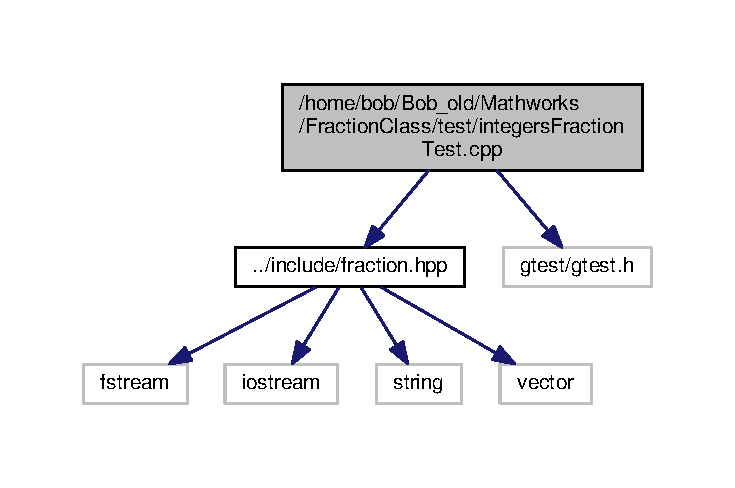
\includegraphics[width=350pt]{integersFractionTest_8cpp__incl}
\end{center}
\end{figure}
\subsection*{Functions}
\begin{DoxyCompactItemize}
\item 
\hyperlink{integersFractionTest_8cpp_a6846e99e1d34a7ffcb0ea6cfefebec92}{T\+E\+ST} (integer\+Test, addition\+\_\+numerator)
\begin{DoxyCompactList}\small\item\em check we can add two fractions \end{DoxyCompactList}\item 
\hyperlink{integersFractionTest_8cpp_adbf89477d00662fbe9146ebd50e54a15}{T\+E\+ST} (integer\+Test, addition\+\_\+denominator)
\begin{DoxyCompactList}\small\item\em check denominator after addition \end{DoxyCompactList}\item 
\hyperlink{integersFractionTest_8cpp_a2e3aedc576cfcc34e5105468510536dc}{T\+E\+ST} (integer\+Test, mixed\+\_\+addition\+\_\+nume)
\begin{DoxyCompactList}\small\item\em check a+5; (fraction$<$\+U$>$ + U) and (U +fraction$<$\+U$>$) \end{DoxyCompactList}\item 
\hyperlink{integersFractionTest_8cpp_acacdb7b30884487e0eb24b1e51fe691b}{T\+E\+ST} (integer\+Test, mixed\+\_\+addition\+\_\+deno)
\begin{DoxyCompactList}\small\item\em check fraction$<$\+U$>$ + u and U+ fraction$<$\+U$>$ \end{DoxyCompactList}\item 
\hyperlink{integersFractionTest_8cpp_a350e9a3cb8d41c2a9cd729207b325113}{T\+E\+ST} (integer\+Test, subtraction\+\_\+numerator)
\begin{DoxyCompactList}\small\item\em check fractions subtraction numerator results \end{DoxyCompactList}\item 
\hyperlink{integersFractionTest_8cpp_a0651a80e023199eab940f9539e6d489e}{T\+E\+ST} (integer\+Test, subtraction\+\_\+deno)
\begin{DoxyCompactList}\small\item\em denominator with Subtraction of two fractions result \end{DoxyCompactList}\item 
\hyperlink{integersFractionTest_8cpp_a665e448356e3bd6b7b0ee055743916d3}{T\+E\+ST} (integer\+Test, mixed\+\_\+sub\+\_\+nume)
\begin{DoxyCompactList}\small\item\em to check fraction$<$\+U$>$ -\/ U $\vert$ U -\/ fraction$<$\+U$>$ \end{DoxyCompactList}\item 
\hyperlink{integersFractionTest_8cpp_a051e428da429f8ae44ab431d6454adfe}{T\+E\+ST} (integer\+Test, mixed\+\_\+sub\+\_\+deno)
\begin{DoxyCompactList}\small\item\em to check fraction$<$\+U$>$ -\/ U $\vert$ U -\/ fraction$<$\+U$>$ result denominator \end{DoxyCompactList}\item 
\hyperlink{integersFractionTest_8cpp_ad678ad5196a46721a1a575540165985c}{T\+E\+ST} (integer\+Test, multiply\+\_\+test)
\begin{DoxyCompactList}\small\item\em product test \end{DoxyCompactList}\item 
\hyperlink{integersFractionTest_8cpp_a9ac7a18bec4855b941ea416d5953160c}{T\+E\+ST} (integer\+Test, multiply\+\_\+mix\+\_\+test)
\begin{DoxyCompactList}\small\item\em Product of U and fraction$<$\+U$>$ \end{DoxyCompactList}\item 
{\bfseries T\+E\+ST} (integer\+Test, divide\+\_\+test)\hypertarget{integersFractionTest_8cpp_a0e5edc9cbba206218c3b8f83ce956f7d}{}\label{integersFractionTest_8cpp_a0e5edc9cbba206218c3b8f83ce956f7d}

\item 
\hyperlink{integersFractionTest_8cpp_a4db3fc7ea226a0bb57a06910c8b273ca}{T\+E\+ST} (integer\+Test, divide\+\_\+mix\+\_\+test)
\begin{DoxyCompactList}\small\item\em check division as fraction$<$\+U$>$ / U ;U/fraction$<$\+U$>$ \end{DoxyCompactList}\item 
\hyperlink{integersFractionTest_8cpp_a02ddd781e2d72f4fa749451b5ccaaaaa}{T\+E\+ST} (integer\+Test, greater\+\_\+test)
\begin{DoxyCompactList}\small\item\em to check which fraction is big \end{DoxyCompactList}\item 
\hyperlink{integersFractionTest_8cpp_a04259b7c50d2092fc0a62518db232130}{T\+E\+ST} (integer\+Test, greater\+\_\+mix\+\_\+test)
\begin{DoxyCompactList}\small\item\em fraction and number comparision \end{DoxyCompactList}\item 
\hyperlink{integersFractionTest_8cpp_a18f7ada1664b3e93e276ba95889e96c5}{T\+E\+ST} (integer\+Test, lesser\+\_\+test)
\begin{DoxyCompactList}\small\item\em to check if $<$ is working \end{DoxyCompactList}\item 
\hyperlink{integersFractionTest_8cpp_a3fde90c692dd1d1c0726321eeb66dfae}{T\+E\+ST} (integer\+Test, lesser\+\_\+mix\+\_\+test)
\begin{DoxyCompactList}\small\item\em checking a/b $<$ c and c $<$ a/b \end{DoxyCompactList}\item 
\hyperlink{integersFractionTest_8cpp_a44f166bb68ce22520ee125b1b875dd08}{T\+E\+ST} (integer\+Test, equality\+\_\+test)
\begin{DoxyCompactList}\small\item\em a/b == c/d fractions equality test \end{DoxyCompactList}\item 
\hyperlink{integersFractionTest_8cpp_aa8cf087f5a8a12c69500cb5d2f8594d2}{T\+E\+ST} (integer\+Test, equality\+Mix\+Test)
\begin{DoxyCompactList}\small\item\em a/b == c; c == a/b \end{DoxyCompactList}\item 
\hyperlink{integersFractionTest_8cpp_a7eb23538d700802489eefb128e07eca7}{T\+E\+ST} (integer\+Test, not\+Equal\+Test)
\begin{DoxyCompactList}\small\item\em a/b !=c/d \end{DoxyCompactList}\item 
\hyperlink{integersFractionTest_8cpp_a10b0fb863dd5cf191d0d8419ddbf611a}{T\+E\+ST} (integer\+Test, not\+Equal\+Mix\+Test)
\begin{DoxyCompactList}\small\item\em a/b!=c;a!=c/d \end{DoxyCompactList}\end{DoxyCompactItemize}
\subsection*{Variables}
\begin{DoxyCompactItemize}
\item 
\hyperlink{classfraction}{fraction}$<$ int $>$ {\bfseries a} (2, 4)\hypertarget{integersFractionTest_8cpp_a343d5b3f8783900052a34d65e514aac6}{}\label{integersFractionTest_8cpp_a343d5b3f8783900052a34d65e514aac6}

\item 
\hyperlink{classfraction}{fraction}$<$ int $>$ {\bfseries b} (6, 8)\hypertarget{integersFractionTest_8cpp_a0a1a5d2a4e9e11fa50b3ad859a93eeda}{}\label{integersFractionTest_8cpp_a0a1a5d2a4e9e11fa50b3ad859a93eeda}

\end{DoxyCompactItemize}


\subsection{Detailed Description}
Includes test cases for all functions in fraction class using int data type. 

\begin{DoxyAuthor}{Author}
Bhargav Dandamudi 
\end{DoxyAuthor}
\begin{DoxyVersion}{Version}
1 
\end{DoxyVersion}
\begin{DoxyDate}{Date}
2019-\/04-\/18 
\end{DoxyDate}


\subsection{Function Documentation}
\index{integers\+Fraction\+Test.\+cpp@{integers\+Fraction\+Test.\+cpp}!T\+E\+ST@{T\+E\+ST}}
\index{T\+E\+ST@{T\+E\+ST}!integers\+Fraction\+Test.\+cpp@{integers\+Fraction\+Test.\+cpp}}
\subsubsection[{\texorpdfstring{T\+E\+S\+T(integer\+Test, addition\+\_\+numerator)}{TEST(integerTest, addition_numerator)}}]{\setlength{\rightskip}{0pt plus 5cm}T\+E\+ST (
\begin{DoxyParamCaption}
\item[{integer\+Test}]{, }
\item[{addition\+\_\+numerator}]{}
\end{DoxyParamCaption}
)}\hypertarget{integersFractionTest_8cpp_a6846e99e1d34a7ffcb0ea6cfefebec92}{}\label{integersFractionTest_8cpp_a6846e99e1d34a7ffcb0ea6cfefebec92}


check we can add two fractions 


\begin{DoxyParams}{Parameters}
{\em integer\+Test} & \\
\hline
{\em addition\+\_\+numerator} & \\
\hline
\end{DoxyParams}
\index{integers\+Fraction\+Test.\+cpp@{integers\+Fraction\+Test.\+cpp}!T\+E\+ST@{T\+E\+ST}}
\index{T\+E\+ST@{T\+E\+ST}!integers\+Fraction\+Test.\+cpp@{integers\+Fraction\+Test.\+cpp}}
\subsubsection[{\texorpdfstring{T\+E\+S\+T(integer\+Test, addition\+\_\+denominator)}{TEST(integerTest, addition_denominator)}}]{\setlength{\rightskip}{0pt plus 5cm}T\+E\+ST (
\begin{DoxyParamCaption}
\item[{integer\+Test}]{, }
\item[{addition\+\_\+denominator}]{}
\end{DoxyParamCaption}
)}\hypertarget{integersFractionTest_8cpp_adbf89477d00662fbe9146ebd50e54a15}{}\label{integersFractionTest_8cpp_adbf89477d00662fbe9146ebd50e54a15}


check denominator after addition 


\begin{DoxyParams}{Parameters}
{\em integer\+Test} & \\
\hline
{\em addition\+\_\+denominator} & \\
\hline
\end{DoxyParams}
\index{integers\+Fraction\+Test.\+cpp@{integers\+Fraction\+Test.\+cpp}!T\+E\+ST@{T\+E\+ST}}
\index{T\+E\+ST@{T\+E\+ST}!integers\+Fraction\+Test.\+cpp@{integers\+Fraction\+Test.\+cpp}}
\subsubsection[{\texorpdfstring{T\+E\+S\+T(integer\+Test, mixed\+\_\+addition\+\_\+nume)}{TEST(integerTest, mixed_addition_nume)}}]{\setlength{\rightskip}{0pt plus 5cm}T\+E\+ST (
\begin{DoxyParamCaption}
\item[{integer\+Test}]{, }
\item[{mixed\+\_\+addition\+\_\+nume}]{}
\end{DoxyParamCaption}
)}\hypertarget{integersFractionTest_8cpp_a2e3aedc576cfcc34e5105468510536dc}{}\label{integersFractionTest_8cpp_a2e3aedc576cfcc34e5105468510536dc}


check a+5; (fraction$<$\+U$>$ + U) and (U +fraction$<$\+U$>$) 


\begin{DoxyParams}{Parameters}
{\em integer\+Test} & \\
\hline
{\em mixed\+\_\+addition\+\_\+nume} & \\
\hline
\end{DoxyParams}
\index{integers\+Fraction\+Test.\+cpp@{integers\+Fraction\+Test.\+cpp}!T\+E\+ST@{T\+E\+ST}}
\index{T\+E\+ST@{T\+E\+ST}!integers\+Fraction\+Test.\+cpp@{integers\+Fraction\+Test.\+cpp}}
\subsubsection[{\texorpdfstring{T\+E\+S\+T(integer\+Test, mixed\+\_\+addition\+\_\+deno)}{TEST(integerTest, mixed_addition_deno)}}]{\setlength{\rightskip}{0pt plus 5cm}T\+E\+ST (
\begin{DoxyParamCaption}
\item[{integer\+Test}]{, }
\item[{mixed\+\_\+addition\+\_\+deno}]{}
\end{DoxyParamCaption}
)}\hypertarget{integersFractionTest_8cpp_acacdb7b30884487e0eb24b1e51fe691b}{}\label{integersFractionTest_8cpp_acacdb7b30884487e0eb24b1e51fe691b}


check fraction$<$\+U$>$ + u and U+ fraction$<$\+U$>$ 


\begin{DoxyParams}{Parameters}
{\em integer\+Test} & \\
\hline
{\em mixed\+\_\+addition\+\_\+deno} & \\
\hline
\end{DoxyParams}
\index{integers\+Fraction\+Test.\+cpp@{integers\+Fraction\+Test.\+cpp}!T\+E\+ST@{T\+E\+ST}}
\index{T\+E\+ST@{T\+E\+ST}!integers\+Fraction\+Test.\+cpp@{integers\+Fraction\+Test.\+cpp}}
\subsubsection[{\texorpdfstring{T\+E\+S\+T(integer\+Test, subtraction\+\_\+numerator)}{TEST(integerTest, subtraction_numerator)}}]{\setlength{\rightskip}{0pt plus 5cm}T\+E\+ST (
\begin{DoxyParamCaption}
\item[{integer\+Test}]{, }
\item[{subtraction\+\_\+numerator}]{}
\end{DoxyParamCaption}
)}\hypertarget{integersFractionTest_8cpp_a350e9a3cb8d41c2a9cd729207b325113}{}\label{integersFractionTest_8cpp_a350e9a3cb8d41c2a9cd729207b325113}


check fractions subtraction numerator results 


\begin{DoxyParams}{Parameters}
{\em integer\+Test} & \\
\hline
{\em subtraction\+\_\+numerator} & \\
\hline
\end{DoxyParams}
\index{integers\+Fraction\+Test.\+cpp@{integers\+Fraction\+Test.\+cpp}!T\+E\+ST@{T\+E\+ST}}
\index{T\+E\+ST@{T\+E\+ST}!integers\+Fraction\+Test.\+cpp@{integers\+Fraction\+Test.\+cpp}}
\subsubsection[{\texorpdfstring{T\+E\+S\+T(integer\+Test, subtraction\+\_\+deno)}{TEST(integerTest, subtraction_deno)}}]{\setlength{\rightskip}{0pt plus 5cm}T\+E\+ST (
\begin{DoxyParamCaption}
\item[{integer\+Test}]{, }
\item[{subtraction\+\_\+deno}]{}
\end{DoxyParamCaption}
)}\hypertarget{integersFractionTest_8cpp_a0651a80e023199eab940f9539e6d489e}{}\label{integersFractionTest_8cpp_a0651a80e023199eab940f9539e6d489e}


denominator with Subtraction of two fractions result 


\begin{DoxyParams}{Parameters}
{\em integer\+Test} & \\
\hline
{\em subtraction\+\_\+deno} & \\
\hline
\end{DoxyParams}
\index{integers\+Fraction\+Test.\+cpp@{integers\+Fraction\+Test.\+cpp}!T\+E\+ST@{T\+E\+ST}}
\index{T\+E\+ST@{T\+E\+ST}!integers\+Fraction\+Test.\+cpp@{integers\+Fraction\+Test.\+cpp}}
\subsubsection[{\texorpdfstring{T\+E\+S\+T(integer\+Test, mixed\+\_\+sub\+\_\+nume)}{TEST(integerTest, mixed_sub_nume)}}]{\setlength{\rightskip}{0pt plus 5cm}T\+E\+ST (
\begin{DoxyParamCaption}
\item[{integer\+Test}]{, }
\item[{mixed\+\_\+sub\+\_\+nume}]{}
\end{DoxyParamCaption}
)}\hypertarget{integersFractionTest_8cpp_a665e448356e3bd6b7b0ee055743916d3}{}\label{integersFractionTest_8cpp_a665e448356e3bd6b7b0ee055743916d3}


to check fraction$<$\+U$>$ -\/ U $\vert$ U -\/ fraction$<$\+U$>$ 


\begin{DoxyParams}{Parameters}
{\em integer\+Test} & \\
\hline
{\em mixed\+\_\+sub\+\_\+nume} & \\
\hline
\end{DoxyParams}
\index{integers\+Fraction\+Test.\+cpp@{integers\+Fraction\+Test.\+cpp}!T\+E\+ST@{T\+E\+ST}}
\index{T\+E\+ST@{T\+E\+ST}!integers\+Fraction\+Test.\+cpp@{integers\+Fraction\+Test.\+cpp}}
\subsubsection[{\texorpdfstring{T\+E\+S\+T(integer\+Test, mixed\+\_\+sub\+\_\+deno)}{TEST(integerTest, mixed_sub_deno)}}]{\setlength{\rightskip}{0pt plus 5cm}T\+E\+ST (
\begin{DoxyParamCaption}
\item[{integer\+Test}]{, }
\item[{mixed\+\_\+sub\+\_\+deno}]{}
\end{DoxyParamCaption}
)}\hypertarget{integersFractionTest_8cpp_a051e428da429f8ae44ab431d6454adfe}{}\label{integersFractionTest_8cpp_a051e428da429f8ae44ab431d6454adfe}


to check fraction$<$\+U$>$ -\/ U $\vert$ U -\/ fraction$<$\+U$>$ result denominator 


\begin{DoxyParams}{Parameters}
{\em integer\+Test} & \\
\hline
{\em mixed\+\_\+sub\+\_\+dino} & \\
\hline
\end{DoxyParams}
\index{integers\+Fraction\+Test.\+cpp@{integers\+Fraction\+Test.\+cpp}!T\+E\+ST@{T\+E\+ST}}
\index{T\+E\+ST@{T\+E\+ST}!integers\+Fraction\+Test.\+cpp@{integers\+Fraction\+Test.\+cpp}}
\subsubsection[{\texorpdfstring{T\+E\+S\+T(integer\+Test, multiply\+\_\+test)}{TEST(integerTest, multiply_test)}}]{\setlength{\rightskip}{0pt plus 5cm}T\+E\+ST (
\begin{DoxyParamCaption}
\item[{integer\+Test}]{, }
\item[{multiply\+\_\+test}]{}
\end{DoxyParamCaption}
)}\hypertarget{integersFractionTest_8cpp_ad678ad5196a46721a1a575540165985c}{}\label{integersFractionTest_8cpp_ad678ad5196a46721a1a575540165985c}


product test 


\begin{DoxyParams}{Parameters}
{\em integer\+Test} & \\
\hline
{\em multiply\+\_\+test} & \\
\hline
\end{DoxyParams}
\index{integers\+Fraction\+Test.\+cpp@{integers\+Fraction\+Test.\+cpp}!T\+E\+ST@{T\+E\+ST}}
\index{T\+E\+ST@{T\+E\+ST}!integers\+Fraction\+Test.\+cpp@{integers\+Fraction\+Test.\+cpp}}
\subsubsection[{\texorpdfstring{T\+E\+S\+T(integer\+Test, multiply\+\_\+mix\+\_\+test)}{TEST(integerTest, multiply_mix_test)}}]{\setlength{\rightskip}{0pt plus 5cm}T\+E\+ST (
\begin{DoxyParamCaption}
\item[{integer\+Test}]{, }
\item[{multiply\+\_\+mix\+\_\+test}]{}
\end{DoxyParamCaption}
)}\hypertarget{integersFractionTest_8cpp_a9ac7a18bec4855b941ea416d5953160c}{}\label{integersFractionTest_8cpp_a9ac7a18bec4855b941ea416d5953160c}


Product of U and fraction$<$\+U$>$ 


\begin{DoxyParams}{Parameters}
{\em integer\+Test} & \\
\hline
{\em multiply\+\_\+mix\+\_\+test} & \\
\hline
\end{DoxyParams}
Division Test


\begin{DoxyParams}{Parameters}
{\em integer\+Test} & \\
\hline
{\em divide\+\_\+test} & \\
\hline
\end{DoxyParams}
\index{integers\+Fraction\+Test.\+cpp@{integers\+Fraction\+Test.\+cpp}!T\+E\+ST@{T\+E\+ST}}
\index{T\+E\+ST@{T\+E\+ST}!integers\+Fraction\+Test.\+cpp@{integers\+Fraction\+Test.\+cpp}}
\subsubsection[{\texorpdfstring{T\+E\+S\+T(integer\+Test, divide\+\_\+mix\+\_\+test)}{TEST(integerTest, divide_mix_test)}}]{\setlength{\rightskip}{0pt plus 5cm}T\+E\+ST (
\begin{DoxyParamCaption}
\item[{integer\+Test}]{, }
\item[{divide\+\_\+mix\+\_\+test}]{}
\end{DoxyParamCaption}
)}\hypertarget{integersFractionTest_8cpp_a4db3fc7ea226a0bb57a06910c8b273ca}{}\label{integersFractionTest_8cpp_a4db3fc7ea226a0bb57a06910c8b273ca}


check division as fraction$<$\+U$>$ / U ;U/fraction$<$\+U$>$ 


\begin{DoxyParams}{Parameters}
{\em integer\+Test} & \\
\hline
{\em divide\+\_\+mix\+\_\+test} & \\
\hline
\end{DoxyParams}
\index{integers\+Fraction\+Test.\+cpp@{integers\+Fraction\+Test.\+cpp}!T\+E\+ST@{T\+E\+ST}}
\index{T\+E\+ST@{T\+E\+ST}!integers\+Fraction\+Test.\+cpp@{integers\+Fraction\+Test.\+cpp}}
\subsubsection[{\texorpdfstring{T\+E\+S\+T(integer\+Test, greater\+\_\+test)}{TEST(integerTest, greater_test)}}]{\setlength{\rightskip}{0pt plus 5cm}T\+E\+ST (
\begin{DoxyParamCaption}
\item[{integer\+Test}]{, }
\item[{greater\+\_\+test}]{}
\end{DoxyParamCaption}
)}\hypertarget{integersFractionTest_8cpp_a02ddd781e2d72f4fa749451b5ccaaaaa}{}\label{integersFractionTest_8cpp_a02ddd781e2d72f4fa749451b5ccaaaaa}


to check which fraction is big 


\begin{DoxyParams}{Parameters}
{\em integer\+Test} & \\
\hline
{\em greater\+\_\+test} & \\
\hline
\end{DoxyParams}
\index{integers\+Fraction\+Test.\+cpp@{integers\+Fraction\+Test.\+cpp}!T\+E\+ST@{T\+E\+ST}}
\index{T\+E\+ST@{T\+E\+ST}!integers\+Fraction\+Test.\+cpp@{integers\+Fraction\+Test.\+cpp}}
\subsubsection[{\texorpdfstring{T\+E\+S\+T(integer\+Test, greater\+\_\+mix\+\_\+test)}{TEST(integerTest, greater_mix_test)}}]{\setlength{\rightskip}{0pt plus 5cm}T\+E\+ST (
\begin{DoxyParamCaption}
\item[{integer\+Test}]{, }
\item[{greater\+\_\+mix\+\_\+test}]{}
\end{DoxyParamCaption}
)}\hypertarget{integersFractionTest_8cpp_a04259b7c50d2092fc0a62518db232130}{}\label{integersFractionTest_8cpp_a04259b7c50d2092fc0a62518db232130}


fraction and number comparision 


\begin{DoxyParams}{Parameters}
{\em integer\+Test} & \\
\hline
{\em greater\+\_\+mix\+\_\+test} & \\
\hline
\end{DoxyParams}
\index{integers\+Fraction\+Test.\+cpp@{integers\+Fraction\+Test.\+cpp}!T\+E\+ST@{T\+E\+ST}}
\index{T\+E\+ST@{T\+E\+ST}!integers\+Fraction\+Test.\+cpp@{integers\+Fraction\+Test.\+cpp}}
\subsubsection[{\texorpdfstring{T\+E\+S\+T(integer\+Test, lesser\+\_\+test)}{TEST(integerTest, lesser_test)}}]{\setlength{\rightskip}{0pt plus 5cm}T\+E\+ST (
\begin{DoxyParamCaption}
\item[{integer\+Test}]{, }
\item[{lesser\+\_\+test}]{}
\end{DoxyParamCaption}
)}\hypertarget{integersFractionTest_8cpp_a18f7ada1664b3e93e276ba95889e96c5}{}\label{integersFractionTest_8cpp_a18f7ada1664b3e93e276ba95889e96c5}


to check if $<$ is working 


\begin{DoxyParams}{Parameters}
{\em integer\+Test} & \\
\hline
{\em lesser\+\_\+test} & \\
\hline
\end{DoxyParams}
\index{integers\+Fraction\+Test.\+cpp@{integers\+Fraction\+Test.\+cpp}!T\+E\+ST@{T\+E\+ST}}
\index{T\+E\+ST@{T\+E\+ST}!integers\+Fraction\+Test.\+cpp@{integers\+Fraction\+Test.\+cpp}}
\subsubsection[{\texorpdfstring{T\+E\+S\+T(integer\+Test, lesser\+\_\+mix\+\_\+test)}{TEST(integerTest, lesser_mix_test)}}]{\setlength{\rightskip}{0pt plus 5cm}T\+E\+ST (
\begin{DoxyParamCaption}
\item[{integer\+Test}]{, }
\item[{lesser\+\_\+mix\+\_\+test}]{}
\end{DoxyParamCaption}
)}\hypertarget{integersFractionTest_8cpp_a3fde90c692dd1d1c0726321eeb66dfae}{}\label{integersFractionTest_8cpp_a3fde90c692dd1d1c0726321eeb66dfae}


checking a/b $<$ c and c $<$ a/b 


\begin{DoxyParams}{Parameters}
{\em integer\+Test} & \\
\hline
{\em lesser\+\_\+mix\+\_\+test} & \\
\hline
\end{DoxyParams}
\index{integers\+Fraction\+Test.\+cpp@{integers\+Fraction\+Test.\+cpp}!T\+E\+ST@{T\+E\+ST}}
\index{T\+E\+ST@{T\+E\+ST}!integers\+Fraction\+Test.\+cpp@{integers\+Fraction\+Test.\+cpp}}
\subsubsection[{\texorpdfstring{T\+E\+S\+T(integer\+Test, equality\+\_\+test)}{TEST(integerTest, equality_test)}}]{\setlength{\rightskip}{0pt plus 5cm}T\+E\+ST (
\begin{DoxyParamCaption}
\item[{integer\+Test}]{, }
\item[{equality\+\_\+test}]{}
\end{DoxyParamCaption}
)}\hypertarget{integersFractionTest_8cpp_a44f166bb68ce22520ee125b1b875dd08}{}\label{integersFractionTest_8cpp_a44f166bb68ce22520ee125b1b875dd08}


a/b == c/d fractions equality test 


\begin{DoxyParams}{Parameters}
{\em integer\+Test} & \\
\hline
{\em equality\+\_\+test} & \\
\hline
\end{DoxyParams}
\index{integers\+Fraction\+Test.\+cpp@{integers\+Fraction\+Test.\+cpp}!T\+E\+ST@{T\+E\+ST}}
\index{T\+E\+ST@{T\+E\+ST}!integers\+Fraction\+Test.\+cpp@{integers\+Fraction\+Test.\+cpp}}
\subsubsection[{\texorpdfstring{T\+E\+S\+T(integer\+Test, equality\+Mix\+Test)}{TEST(integerTest, equalityMixTest)}}]{\setlength{\rightskip}{0pt plus 5cm}T\+E\+ST (
\begin{DoxyParamCaption}
\item[{integer\+Test}]{, }
\item[{equality\+Mix\+Test}]{}
\end{DoxyParamCaption}
)}\hypertarget{integersFractionTest_8cpp_aa8cf087f5a8a12c69500cb5d2f8594d2}{}\label{integersFractionTest_8cpp_aa8cf087f5a8a12c69500cb5d2f8594d2}


a/b == c; c == a/b 


\begin{DoxyParams}{Parameters}
{\em integer\+Test} & \\
\hline
{\em equality\+Mix\+Test} & \\
\hline
\end{DoxyParams}
\index{integers\+Fraction\+Test.\+cpp@{integers\+Fraction\+Test.\+cpp}!T\+E\+ST@{T\+E\+ST}}
\index{T\+E\+ST@{T\+E\+ST}!integers\+Fraction\+Test.\+cpp@{integers\+Fraction\+Test.\+cpp}}
\subsubsection[{\texorpdfstring{T\+E\+S\+T(integer\+Test, not\+Equal\+Test)}{TEST(integerTest, notEqualTest)}}]{\setlength{\rightskip}{0pt plus 5cm}T\+E\+ST (
\begin{DoxyParamCaption}
\item[{integer\+Test}]{, }
\item[{not\+Equal\+Test}]{}
\end{DoxyParamCaption}
)}\hypertarget{integersFractionTest_8cpp_a7eb23538d700802489eefb128e07eca7}{}\label{integersFractionTest_8cpp_a7eb23538d700802489eefb128e07eca7}


a/b !=c/d 


\begin{DoxyParams}{Parameters}
{\em integer\+Test} & \\
\hline
{\em not\+Equal\+Test} & \\
\hline
\end{DoxyParams}
\index{integers\+Fraction\+Test.\+cpp@{integers\+Fraction\+Test.\+cpp}!T\+E\+ST@{T\+E\+ST}}
\index{T\+E\+ST@{T\+E\+ST}!integers\+Fraction\+Test.\+cpp@{integers\+Fraction\+Test.\+cpp}}
\subsubsection[{\texorpdfstring{T\+E\+S\+T(integer\+Test, not\+Equal\+Mix\+Test)}{TEST(integerTest, notEqualMixTest)}}]{\setlength{\rightskip}{0pt plus 5cm}T\+E\+ST (
\begin{DoxyParamCaption}
\item[{integer\+Test}]{, }
\item[{not\+Equal\+Mix\+Test}]{}
\end{DoxyParamCaption}
)}\hypertarget{integersFractionTest_8cpp_a10b0fb863dd5cf191d0d8419ddbf611a}{}\label{integersFractionTest_8cpp_a10b0fb863dd5cf191d0d8419ddbf611a}


a/b!=c;a!=c/d 


\begin{DoxyParams}{Parameters}
{\em integer\+Test} & \\
\hline
{\em not\+Equal\+Mix\+Test} & \\
\hline
\end{DoxyParams}

%--- End generated contents ---

% Index
\backmatter
\newpage
\phantomsection
\clearemptydoublepage
\addcontentsline{toc}{chapter}{Index}
\printindex

\end{document}
